\newcommand*{\DSEIcon}{
\includegraphics[height=0.8em]{figures/dse/DSEIcon}}%
\newcommand*{\ResultsIcon}{
\includegraphics[height=0.8em]{figures/dse/results-actualIcon}}%
%
%
%
\section{Design Space Exploration}\label{sec:DSE}
This section provides a description of \into tool chain support for design space exploration (DSE.)
%
%
This section is split into four parts.  In Section~\ref{sec:dse:install} the installation procedure is outlined. Section~\ref{sec:dse:launch} describes how the \intoapp{} can be used to launch a DSE using an existing configuration file and Section~\ref{sec:dse:results} describes how the results from DSE are generated and stored.  Section~\ref{sec:dse:edit} describes the structure of the DSE configuration file, giving enough detail for the user to be able to edit one for their purposes.
%
%
%
\subsection{Installing DSE Scripts}\label{sec:dse:install}
Before we launch a  DSE, we must install the DSE scripts for the various search algorithms and objective evaluation. In the  \intoapp{}, select  \textit{Window} $\rightarrow$ \textit{Show Download Manager}. This opens the download manager as shown in Figure~\ref{fig:dse:download_mngr}. Select the most recent release and download \textit{Design Space Exploration - Scripts for generating and analysing multiple co-simulations}.
%
Python version 2.7 must be installed, along with the matplotlib library.

\begin{figure}[ht]
	\centering
	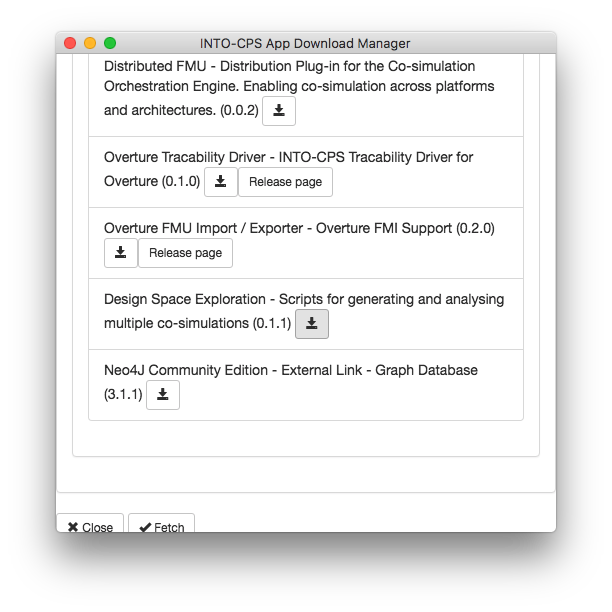
\includegraphics[width=0.7\textwidth]{figures/dse/download_mngr}
	\caption{Download Manager.}\label{fig:dse:download_mngr}
\end{figure}

This will download a Zip archive -- extract this into the directory in which the archive was downloaded. DSEs may now be launched.

\subsection{How to Launch a DSE}\label{sec:dse:launch}
To launch a DSE we need to provide the \intoapp{} with the path to two files.  The first is the DSE configuration, defining the parameters of the design space, how it should be searched, measured and the results compared.   The second is the multi-model configuration, defining the base model that will be used for the search.  A DSE configuration is selected by double clicking on one of the configurations listed in the \emph{DSES} section of the \intoapp{} project explorer; these configurations are identified with the (\DSEIcon) icon.  Hint: several of the downloadable examples have predefined  DSE configurations.

To launch the DSE, we must first select the multi-model to use. One can be selected by clicking the \emph{Set multi-model} button and selecting one from the drop-down list, as shown in Figures \ref{fig:dse:launch:selectmultimodel} and \ref{fig:dse:launch:setmultimodel}.  Once selected, your choice must be saved to parse the DSE configuration with respect to the multi-model of choice by clicking on the \emph{Save multi-model choice} button, as shown in Figure~\ref{fig:dse:launch:setmultimodel}.
%
%
%
\begin{figure}
	\centering
	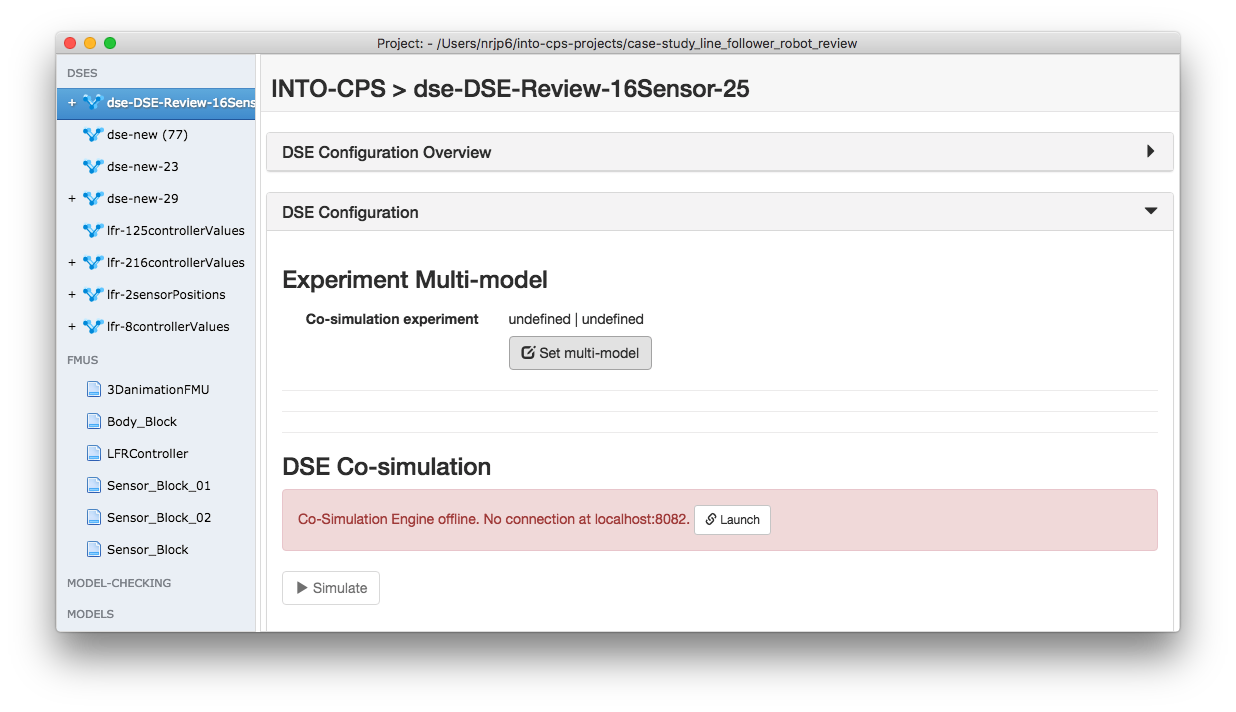
\includegraphics[width=0.8\textwidth]{figures/dse/launch-selectmultimodel}
	\caption{Selecting a multi-model.}\label{fig:dse:launch:selectmultimodel}
\end{figure}

\begin{figure}
	\centering
	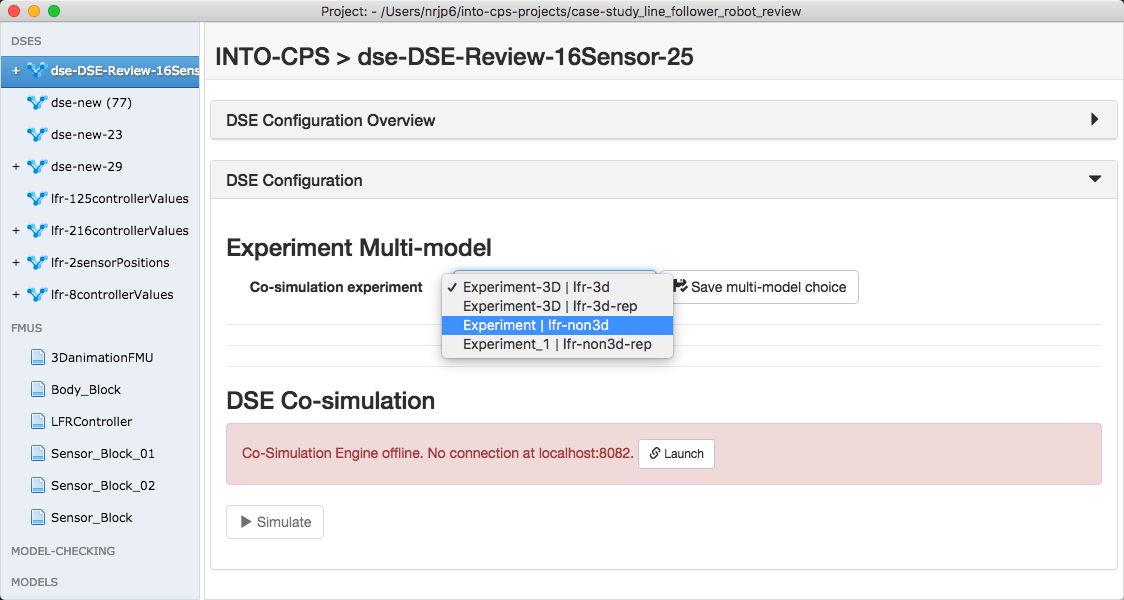
\includegraphics[width=0.8\textwidth]{figures/dse/launch-setmultimodel}
	\caption{Setting a multi-model.}\label{fig:dse:launch:setmultimodel}
\end{figure}

If the COE is not already running, the bottom of the DSE page is shown with a red ``\emph{Co-Simulation Engine offline. No connection at localhost:8082}'' status, as shown in Figure \ref{fig:dse:launch:dsesection}.
%
If this is the case, click on the \emph{Launch} button to start the COE.
%
This results in a green co-simulation engine status (see Figure \ref{fig:dse:launch:coerunning}). Pressing the \emph{Simulate} button starts the DSE background process.
%
%
%
\begin{figure}[ht]
	\centering
	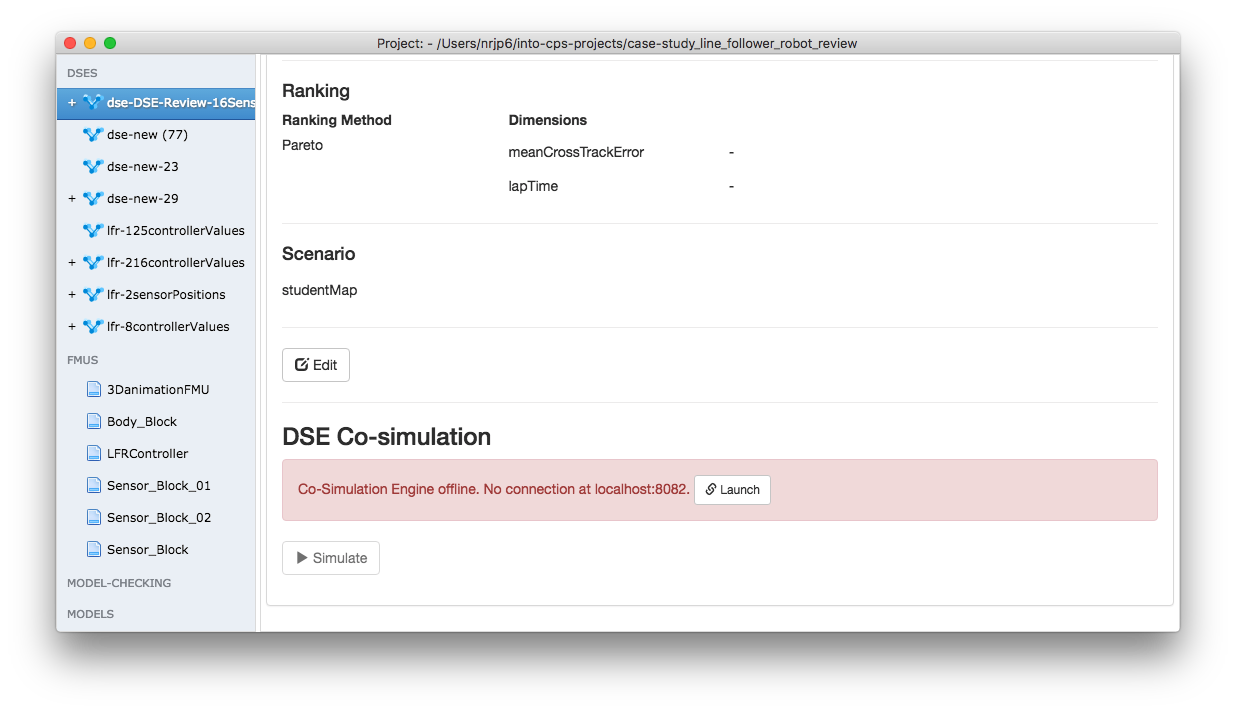
\includegraphics[width=0.9\textwidth]{figures/dse/launch-dsesection}
	\caption{Status when COE is not running.}\label{fig:dse:launch:dsesection}
\end{figure}
%
%
%
\begin{figure}[ht]
	\centering
	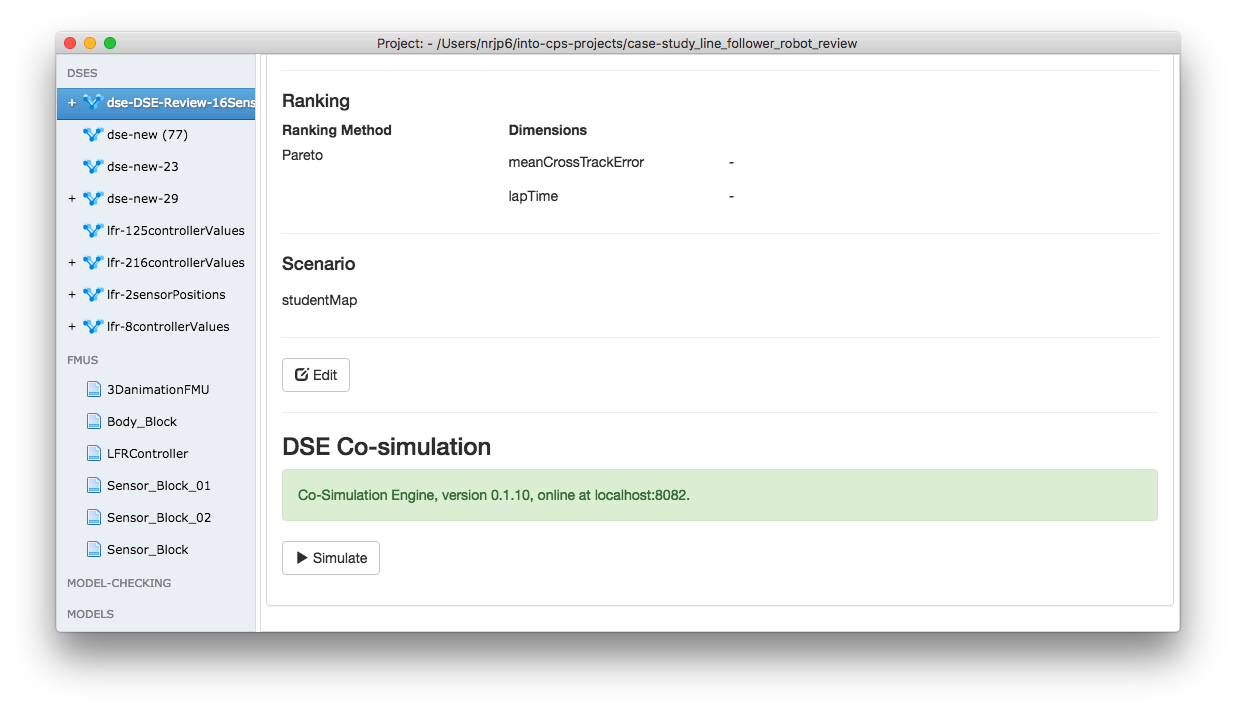
\includegraphics[width=0.8\textwidth]{figures/dse/launch-coerunning}
	\caption{Status when COE is running.}\label{fig:dse:launch:coerunning}
\end{figure}
%
%
%
%With the DSE configuration selected and the COE running, the next step is to select the multi-model to use.
%
%One can be selected from the \emph{Co-simulation Configuration} drop-down box, as shown in Figure \ref{fig:dse:launch:selectmultimodel}.  Pressing the \emph{Simulate} button starts the DSE background process.
%
%
%
\subsection{Results of a DSE}\label{sec:dse:results}
The DSE scripts store their results in a folder named for the date and time at which the DSE was started.
%
This folder may be found underneath the name of the DSE script selected, as shown in Figure~\ref{fig:dse:results:icon}.  When the DSE has finished, we can find both a graphs folder and an HTML results page inside the results folder.
%
It may be necessary to refresh the project view to see these new items.  The results HTML file is identified by the (\ResultsIcon) icon, and double clicking on it opens the results page in the computer's default browser.
%
%
%
\begin{figure}[ht]
	\centering
	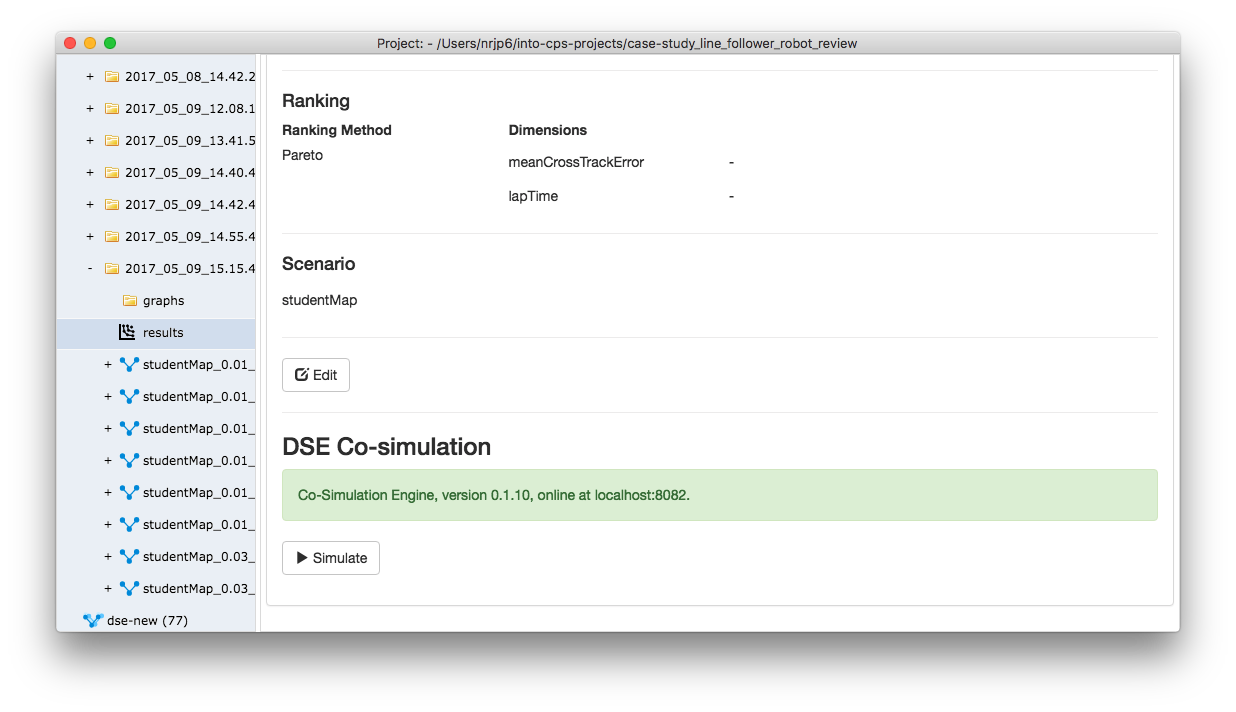
\includegraphics[width=0.8\textwidth]{figures/dse/results-icon}
	\caption{Icon shown when DSE results are ready.}\label{fig:dse:results:icon}
\end{figure}
%
%
%

The results, shown in Figure~\ref{fig:dse:results:page}, contain two elements.  The first element is a Pareto graph showing the results of all simulations on a single plot, with each point on the graph representing a single simulation.  The best designs, referred to as the non-dominated set, are shown in blue, with ranks of progressively worse designs coloured alternately red and yellow.  The second element is a table of these results, with the rank in the left hand column, followed by the objective values and finally the design parameters that produced the result.
%
%
%
\begin{figure}[ht]
	\centering
	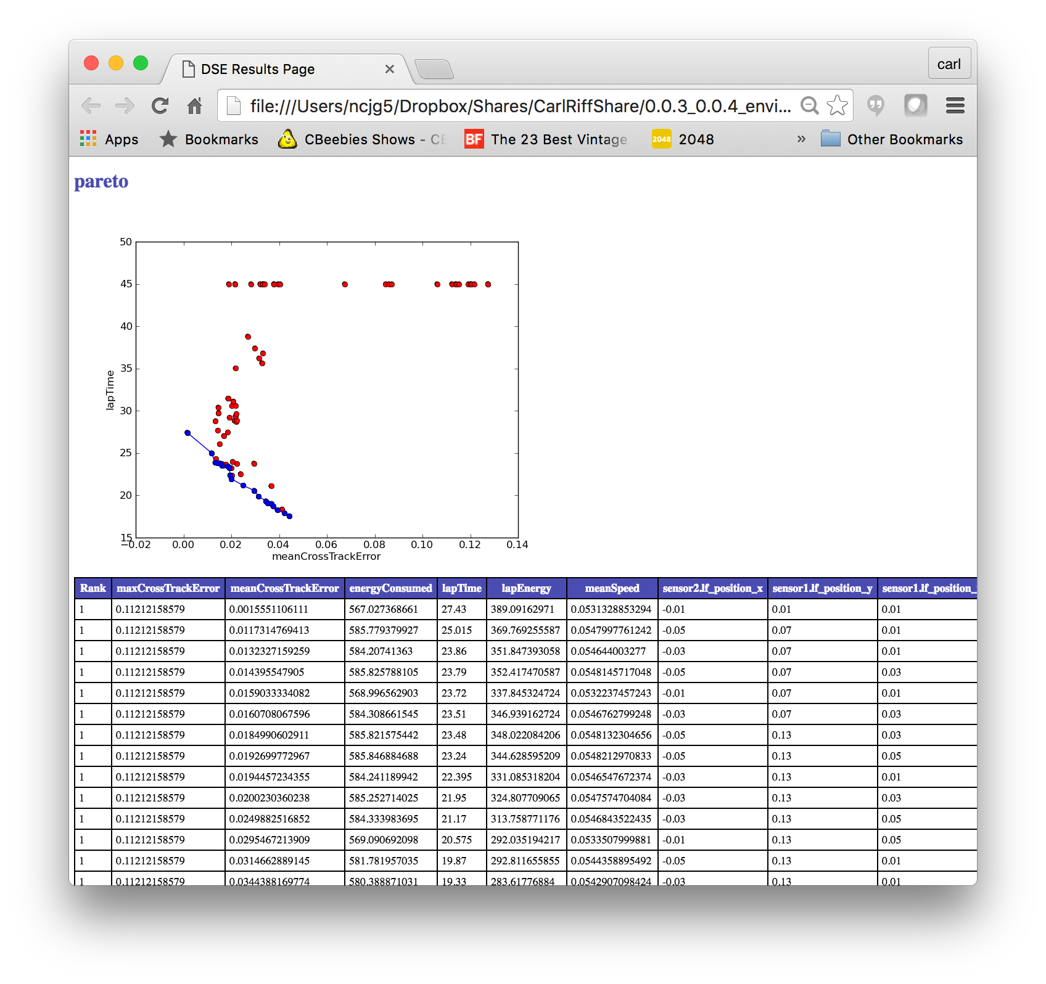
\includegraphics[width=\textwidth]{figures/dse/results-page}
	\caption{A page of DSE results.}\label{fig:dse:results:page}
\end{figure}
%
%
%
\subsection{How to Edit a DSE Configuration}\label{sec:dse:edit}

A DSE configuration comprises several elements. In Section~\ref{sec:dse:overview} we outline the content of each element and their role in a DSE. 
There are three methods for producing DSE configurations; through the use of the INTO-SysML DSE profile (Section~\ref{sec:dse:edit:sysml}), through the \intoapp{} (this method may also be used to edit an existing configuration) (Section~\ref{sec:dse:edit:app}), or manually editing a text configuration document (Section~\ref{sec:dse:edit:manual}). In this section we outline each approach.  



\subsubsection{DSE Configuration Overview}\label{sec:dse:overview}

A DSE configuration comprises several elements: the search algorithm to use; parameters; parameter constraints; objectives; objective constraints; a ranking; and a set of scenarios.


\subsubsection*{Search Algorithm}\label{sec:dse:overview:algorithm}

The algorithm section allows a user to choose between DSE search algorithms implemented in INTO-CPS. There are two options at present: \textit{exhaustive} and \textit{genetic}. The exhaustive approach will simulate the whole design space as dictated by the choice of parameters and scenarios. The genetic algorithm uses an approach to selecting the designs to simulate based upon genetic breeding and mutations. For more information on the search algorithms, see Deliverable D3.2a~\cite{INTOCPSD3.2a}.

\subsubsection*{Parameters}\label{sec:dse:overview:parameters}

The parameters section is used to define a list of values for each parameter to be explored.   If a parameter is included in the DSE configuration file, then it must have at least one value defined.  The order of the values in the list is not important. 

\subsubsection*{Parameter Constraints}\label{sec:dse:overview:parameterconstraints}
It may be the case that not all combinations of the parameter values defined in the previous section are valid.
%
So, it is necessary to be able to define constraints over the design parameters such that no time is wasted simulating invalid designs.  For example, in the Line Follower Robot project \cite{INTOCPSD3.6} we define ranges for the x and y co-ordinates of the left and right sensors separately, and running all combinations of these leads to asymmetric designs that do not have the same turning behaviour on left and right turns.  To prevent this we can define boolean expressions based upon the design parameters and evaluate these before a simulation is launched.

\subsubsection*{Objective Definitions: Internal}\label{sec:dse:overview:objectivesinternal}
There are two means for defining the objectives used to assess the performance of a simulated model.  The first of these, described here, is using the internal functions included in the DSE scripts.  This is a set of simple functions that can be applied to any of the values recorded by the COE during simulation.  The current set of internal functions is:
%
%
%
\begin{description}
	\item[max] Returns the maximum value of a variable during a simulation.
	\item[min] Returns the minimum value of a variable during a simulation.
	\item[mean] Returns the mean value of a variable during a simulation (\emph{n.\@b.\@}, a fixed simulation step size is assumed.)
\end{description}
%
%

\subsubsection*{Objective Definitions: External Scripts}\label{sec:dse:overview:objectivesexternal}

The second form of objective definition makes use of user-defined Python scripts to allow bespoke analysis of simulation results to be launched automatically and results recorded using the common format.  The definition has two parts: the construction of the Python script to perform the analysis and the definition of the script's required parameters in the DSE configuration file.  These two steps are described below.

\paragraph{Construction of the Script}

The outline functionality of an analysis script is that, at the appropriate times, a DSE script calls it, passing four or more arguments.  The script uses these arguments to locate a raw simulation results file (\texttt{results.csv}), process those results and then write the objective values into an objectives file (\texttt{objectives.json}) for that simulation.  

The first three arguments sent to the script are common to all scripts.  These are listed below.
%
%
%
\begin{description}
	\item[argv 1 ] The absolute path to the folder containing the \texttt{results.csv} results file.  This is also the path where the script finds the \newline \texttt{objectives.json} file.
	\item[argv 2 ] The name of the objective.  This is the key against which the script should save its results in the objectives file.
	\item[argv 3 ] The name of the scenario.
\end{description}
%
%
%
With this information the script can find the raw simulation data and also determine where to save its results.  The name of the scenario allows the script to locate any data files it needs relating to the scenario.  For example, in the case of the script measuring cross track error for the line following robot, the script makes use of a data file that contains a series of coordinates that represent the line to be followed.  The name of this data file is \texttt{map1px.csv}.  It is placed into a folder with the same name as the scenario, which in this case is \texttt{student\-Map}.  That folder is located in the \texttt{user\-Metric\-Scripts} folder, as shown in Figure~\ref{fig:dse:externalAnalysisDataLocation}.  Using this method, the developer of an external analysis script needs only to define the name of the data file they will need and know that at runtime the script will be passed a path to a folder containing the data file suitable for the scenario under test.
%
%
%
\begin{figure}[ht]
	\centering
	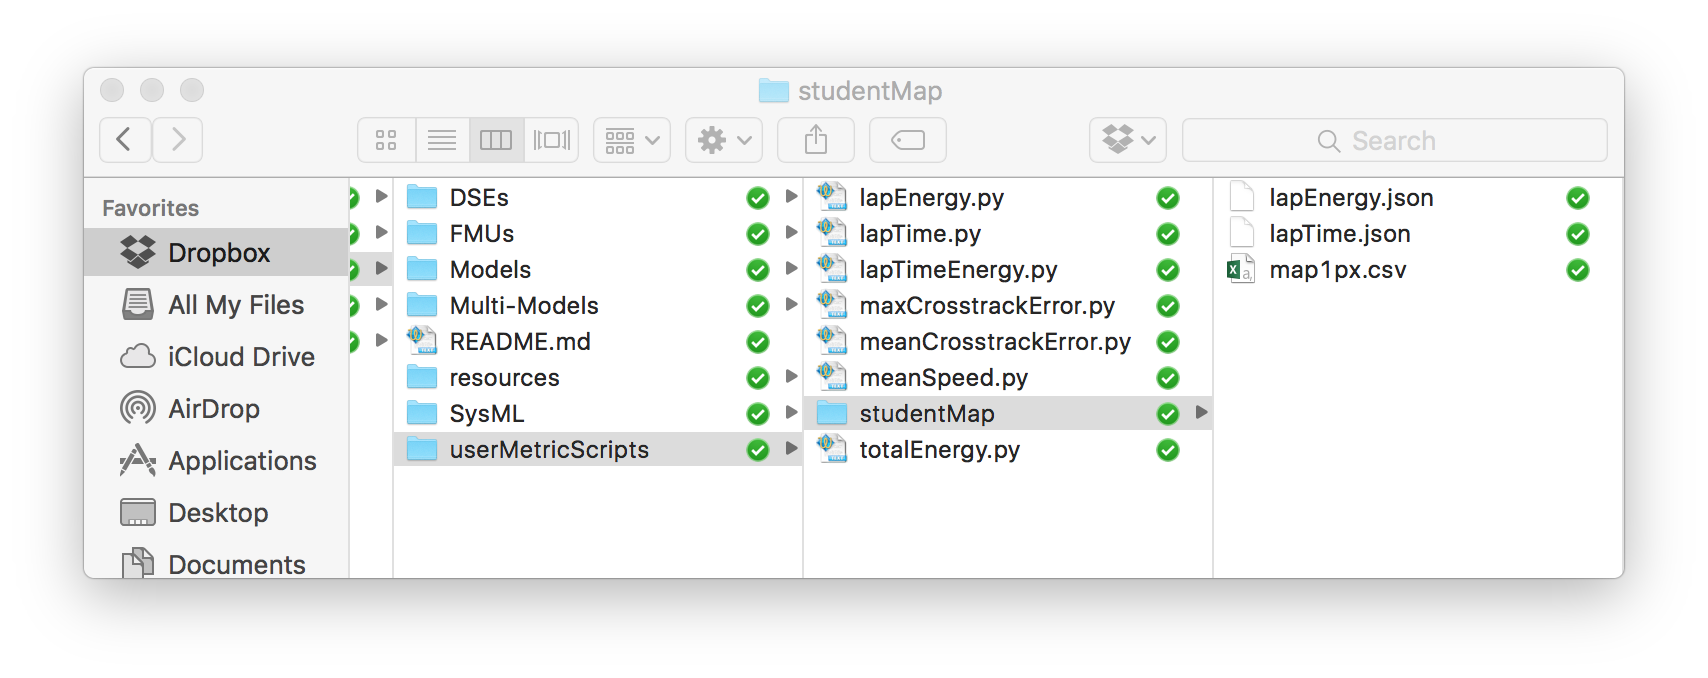
\includegraphics[width=\textwidth]{figures/dse/externalAnalysisDataLocation}
	\caption{External analysis script data files for the ``studentMap'' scenario.}\label{fig:dse:externalAnalysisDataLocation}
\end{figure}

\begin{figure}
	\centering
	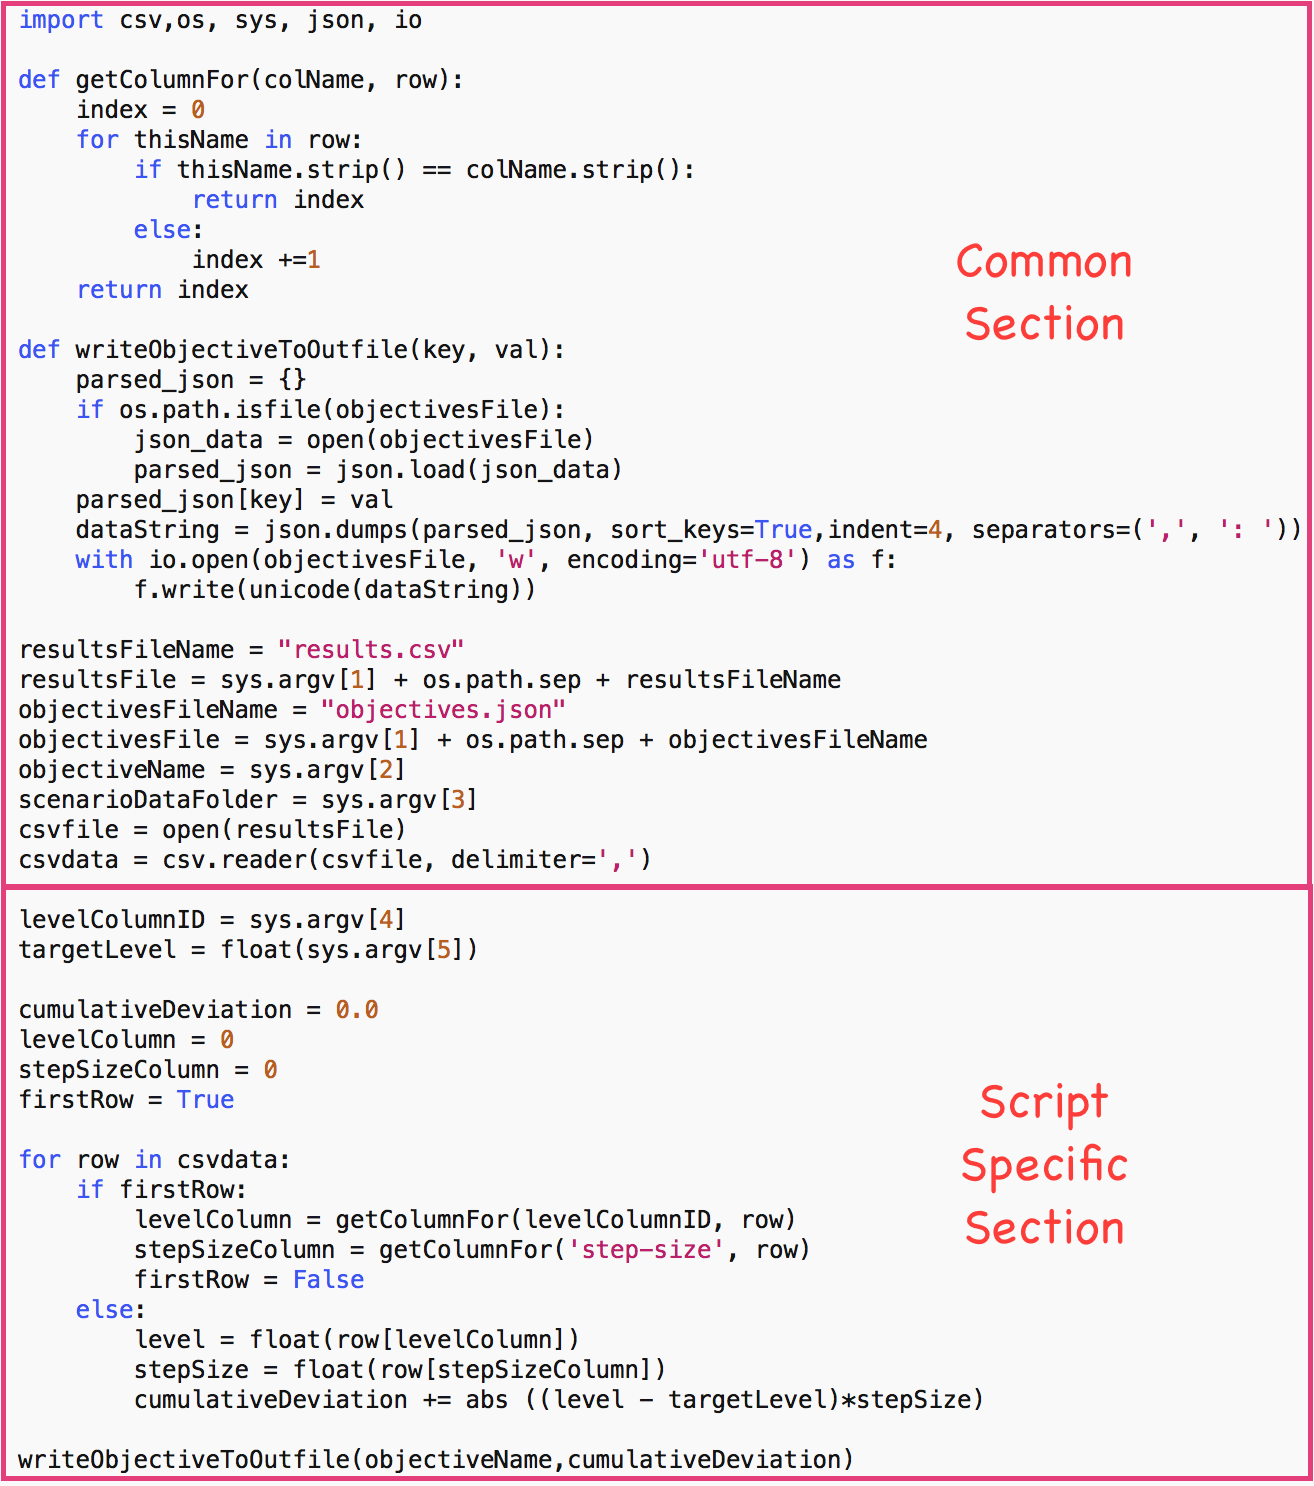
\includegraphics[scale=0.55]{figures/dse/cumulativeDeviationWholeScript}
	\caption{External analysis script to calculate cumulative deviation in the Water Tank example.}\label{fig:dse:edit:cumulativeDeviationWholeScript}
\end{figure}


Figure~\ref{fig:dse:edit:cumulativeDeviationWholeScript} shows an example of an external analysis script.  In this case it computes the cumulative deviation of the water level from some target level.  There are two distinct sections in the file, we shall refer to them as the ``common'' and ``script specific'' sections.  

The common section contains core functions that are common to all external scripts.  It reads in the three arguments that are common to all scripts, and contains functions to help the user retrieve the data needed by the analysis script, and to write the computed objective value into the \texttt{objectives.json} file.  It is recommended that this section be copied to form the basis of any new external analysis scripts.

The second part of the example script shown is specific to the analysis to be performed.  The purpose of this section is to actually compute the value of the objective from the results of a simulation.  Generally it will have three parts: reading in any analysis specific arguments such as the ID of data in the results that it needs, using the data in \texttt{results.csv} to calculate the value of the objective and finally write the objective value into \texttt{objectives.json}.

In the `Script Specific Section' of Figure~\ref{fig:dse:edit:cumulativeDeviationWholeScript} we see the example of the script calculating the cumulative deviation of the water level from a target level in the water tank model.  It starts by reading a further two arguments passed when the script is launched and initializes the variables.  The script then iterates through all rows of data in \texttt{results.csv} to calculate the cumulative deviation which is then written to the \texttt{objectives.json} file in the final line.
%
%
%
\subsubsection*{Ranking}\label{sec:dse:overview:ranking}
The final part of a DSE configuration file concerns the placing of designs in a partial order according to their performance.  The DSE currently supports a Pareto method of ranking, as was shown earlier in Figure~\ref{fig:dse:results:page}.  The purpose of the ranking section of the configuration is to define the pair of objectives that will be used to rank the designs, and whether to maximise or minimise each.  

\subsubsection*{Scenario List}\label{sec:dse:overview:scenarios}
The DSE scripts currently have limited support for scenarios referring to a specific set of conditions against which the multi-model is to be tested.  In the example of the line following robot, the scenario refers to the map the robot has to follow, along with its starting co-ordinates.
%
For instance, in one scenario the robot would go around a circular track in one direction, predominantly turning left, whereas in a different scenario the same track would be followed in the opposite direction, predominantly turning right.
%
In both scenarios the map of the track is the same.


%
%
%


\subsubsection{Using the INTO-SysML DSE Profile}\label{sec:dse:edit:sysml}


The INTO-CPS DSE SysML profile is defined in Deliverable D4.2c~\cite{INTOCPSD4.2c}, with an example of its use in Deliverable D3.3a~\cite{INTOCPSD3.3a}. Here we describe the steps to export the configuration from Modelio and import it into the \intoapp{}.

Given a complete DSE SysML model, as shown in Figure~\ref{fig:dse:edit:sysml}, we generate a DSE configuration by right-clicking on the \texttt{DSEAnalysis} object in the model browser and selecting \textit{INTO-CPS} $\rightarrow$ \textit{GenerateDSE}, as in Figure~\ref{fig:dse:edit:sysml-generate-menu}.
%
%
%
\begin{figure}[ht]
	\centering
	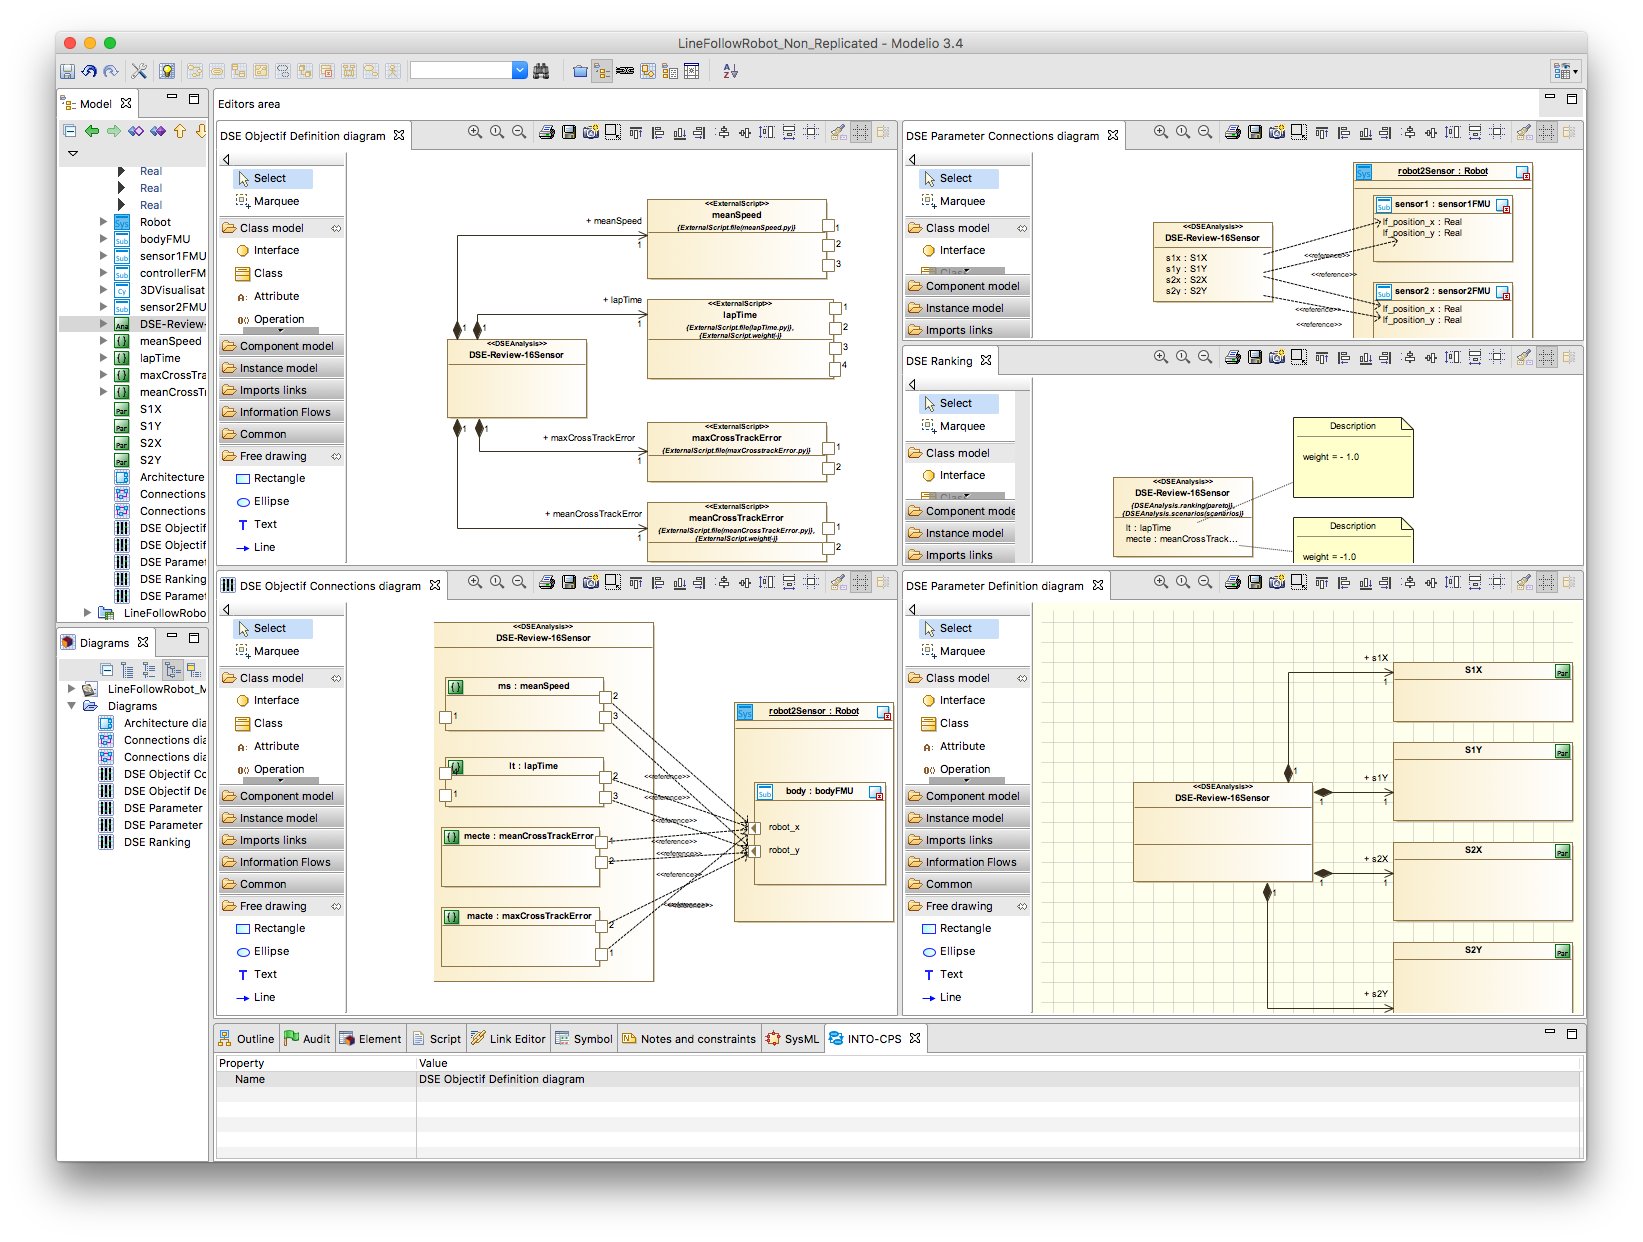
\includegraphics[width=\textwidth]{figures/dse/sysml-model}
	\caption{SysML model of DSE analysis experiment.}\label{fig:dse:edit:sysml}
\end{figure}
%
%
%
\begin{figure}[ht]
	\centering
	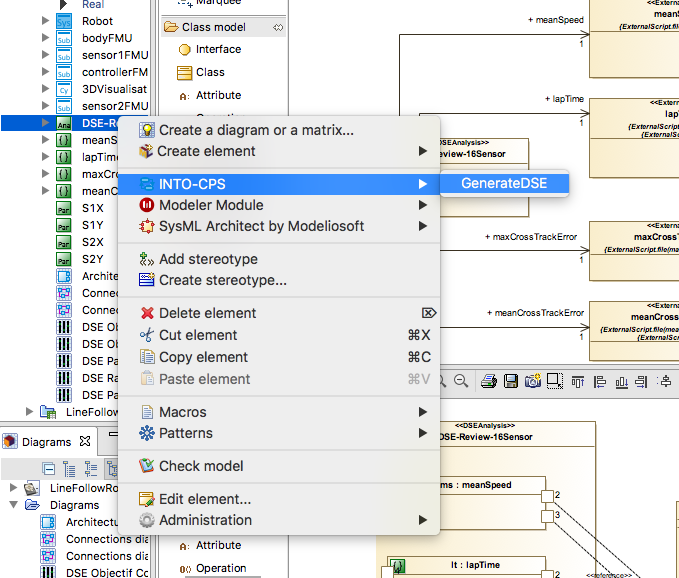
\includegraphics[width=0.6\textwidth]{figures/dse/sysml-generate-menu}
	\caption{Menu option for generating DSE configuration.}\label{fig:dse:edit:sysml-generate-menu}
\end{figure}
%
%
%

Simply supply an appropriate name and select \textit{Export} (Figure~\ref{fig:dse:edit:sysml-generate-name2}). When the export is complete, click \textit{OK} (Figure~\ref{fig:dse:edit:sysml-generate-complete}).
%
%
%
\begin{figure}[ht]
	\centering
	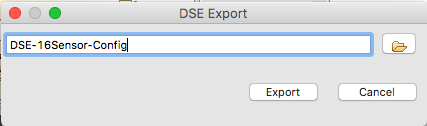
\includegraphics[width=0.5\textwidth]{figures/dse/sysml-generate-name2}
	\caption{Enter DSE configuration name.}\label{fig:dse:edit:sysml-generate-name2}
\end{figure}
%
%
%
\begin{figure}[ht]
	\centering
	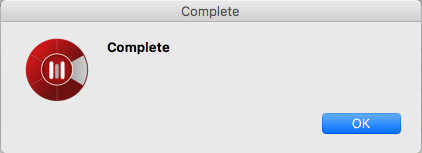
\includegraphics[width=0.5\textwidth]{figures/dse/sysml-generate-complete}
	\caption{Export complete.}\label{fig:dse:edit:sysml-generate-complete}
\end{figure}
%
%
%

Moving to the \intoapp{}, we start to import the configuration. Expand the generated configurations in project's SysML model: \textit{Model}  $\rightarrow$ \textit{configs}, right click on the configuration name as defined above and select \textit{Create DSE Configuration} (see Figure~\ref{fig:dse:edit:sysml-app-menu}). When complete, the configuration screen is displayed, and can be launched according to instructions in Section~\ref{sec:dse:launch}.
%
%
%
\begin{figure}[ht]
	\centering
	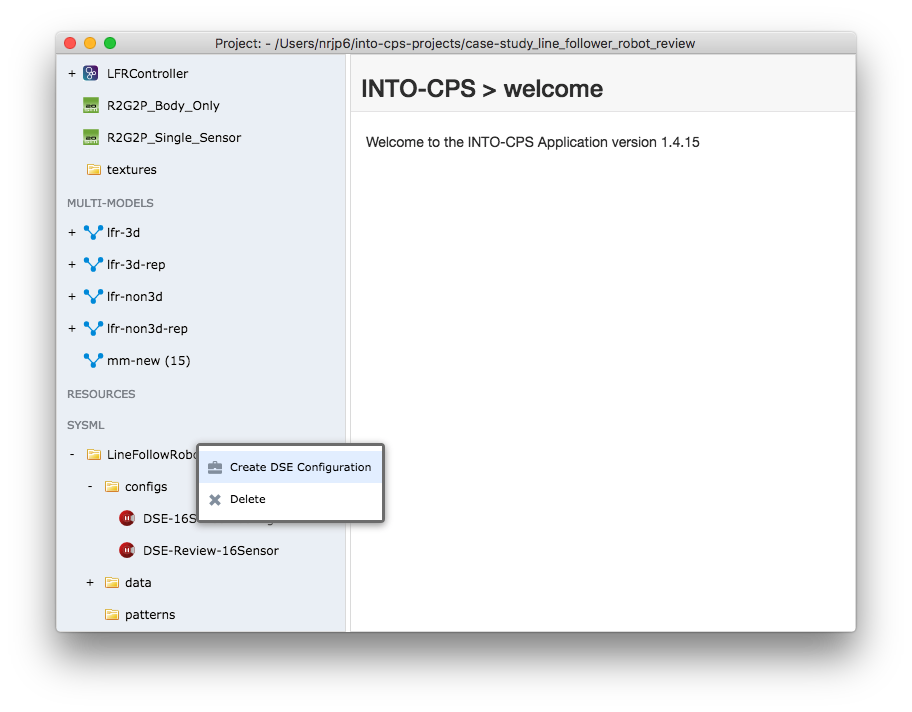
\includegraphics[width=\textwidth]{figures/dse/sysml-app-menu}
	\caption{Create configuration in \intoapp{}.}\label{fig:dse:edit:sysml-app-menu}
\end{figure}
\clearpage




\subsubsection{Using the \intoapp{} DSE Editor}\label{sec:dse:edit:app}

To create a new DSE configuration in the \intoapp{}, right click on the DSES section of the project browser and select \textit{Create Design Space Exploration Config}, as in Figure~\ref{fig:dse:edit:app-create-config}. This will create a new configuration with a name in the form \texttt{dse-new(xx)} with a random number. This can be renamed by right-clicking on the new config in the project browser.
%
\begin{figure}[ht]
	\centering
	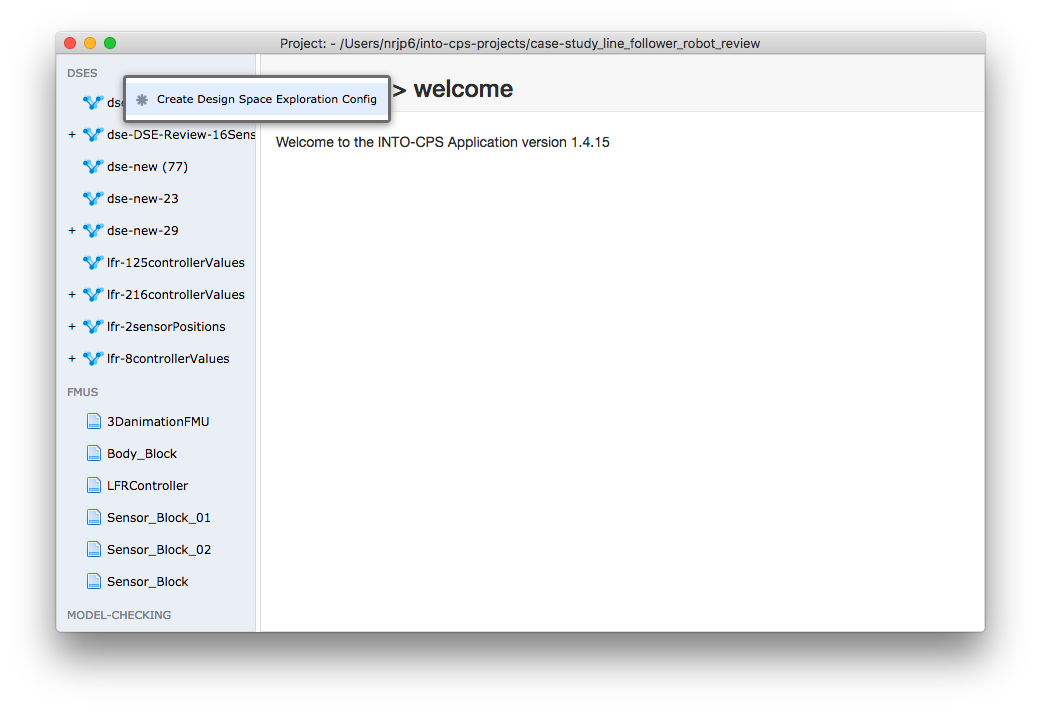
\includegraphics[width=\textwidth]{figures/dse/app-create-config}
	\caption{Create new DSE configuration.}\label{fig:dse:edit:app-create-config}
\end{figure}
%
%
When opened, one must first select the multi-model to use. Follow the same steps as given earlier for launching a DSE (Figures~\ref{fig:dse:launch:selectmultimodel} and~\ref{fig:dse:launch:setmultimodel}). When selected, the DSE configuration may be edited. 

\subsubsection{Search Algorithm}\label{sec:dse:app:algorithm}

The first element to define is the search algorithm. A choice is given between \textit{Exhaustive} and \textit{Genetic} searches, as shown in Figure~\ref{fig:dse:edit:app-algorithm-choice}. The exhaustive option has no further options, whist a genetic search requires data concerning: the \textit{initial population}; \textit{initial population distribution}; \textit{mutation probability}; \textit{parent selection strategy}; and \textit{maximum generations without improvement} -- these are shown in Figure~\ref{fig:dse:edit:app-algorithm-genetic}.
%
%
\begin{figure}[ht]
	\centering
	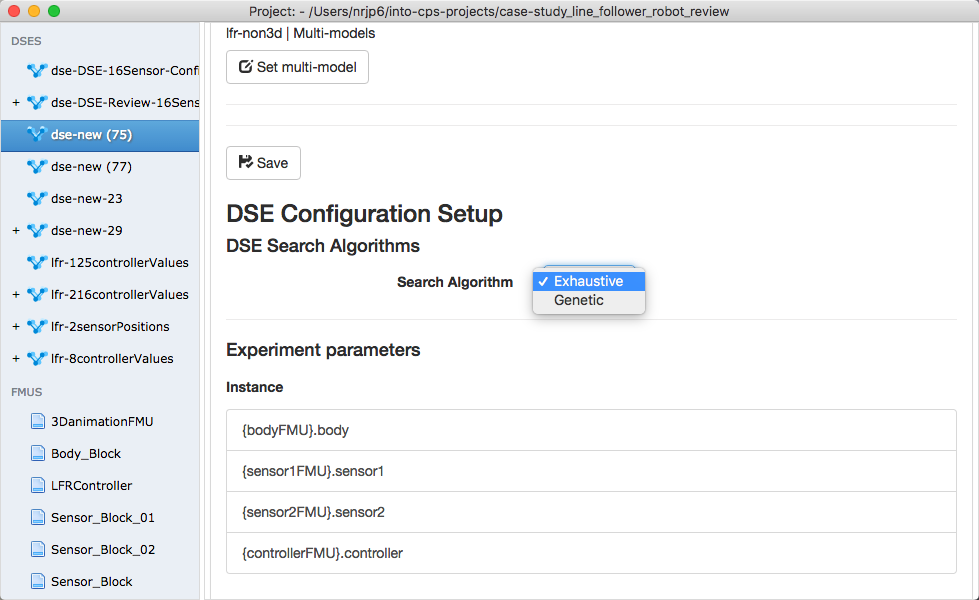
\includegraphics[width=0.9\textwidth]{figures/dse/app-algorithm-choice}
	\caption{Choosing the DSE search algorithm.}\label{fig:dse:edit:app-algorithm-choice}
\end{figure}
%
%
\begin{figure}[ht]
	\centering
	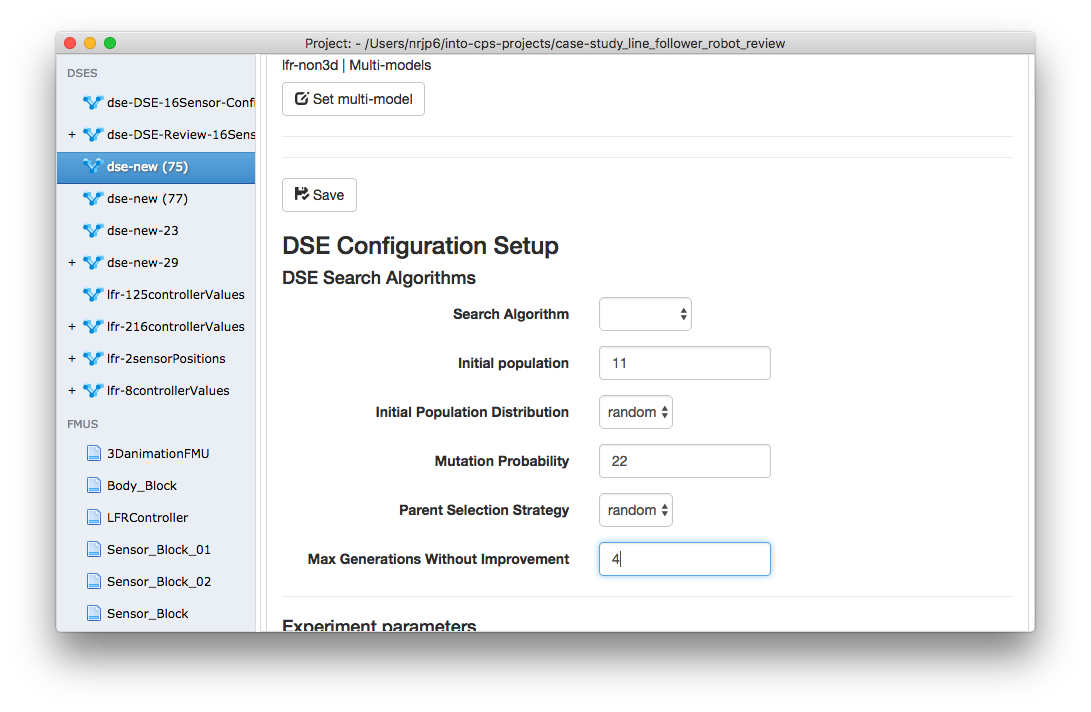
\includegraphics[width=0.9\textwidth]{figures/dse/app-algorithm-genetic}
	\caption{Options for the genetic algorithm.}\label{fig:dse:edit:app-algorithm-genetic}
\end{figure}

\subsubsection{Parameters}\label{sec:dse:app:parameters}

Design parameters may be defined in a multi-model. In addition, a DSE configuration may define a range of values to be used in the DSE. The DSE editor allows users to browse the multi-model parameters (Figure~\ref{fig:dse:edit:app-param}) and edit those parameters defined in the multi-model (Figure~\ref{fig:dse:edit:app-param-edit}). 
%
%
\begin{figure}[ht]
	\centering
	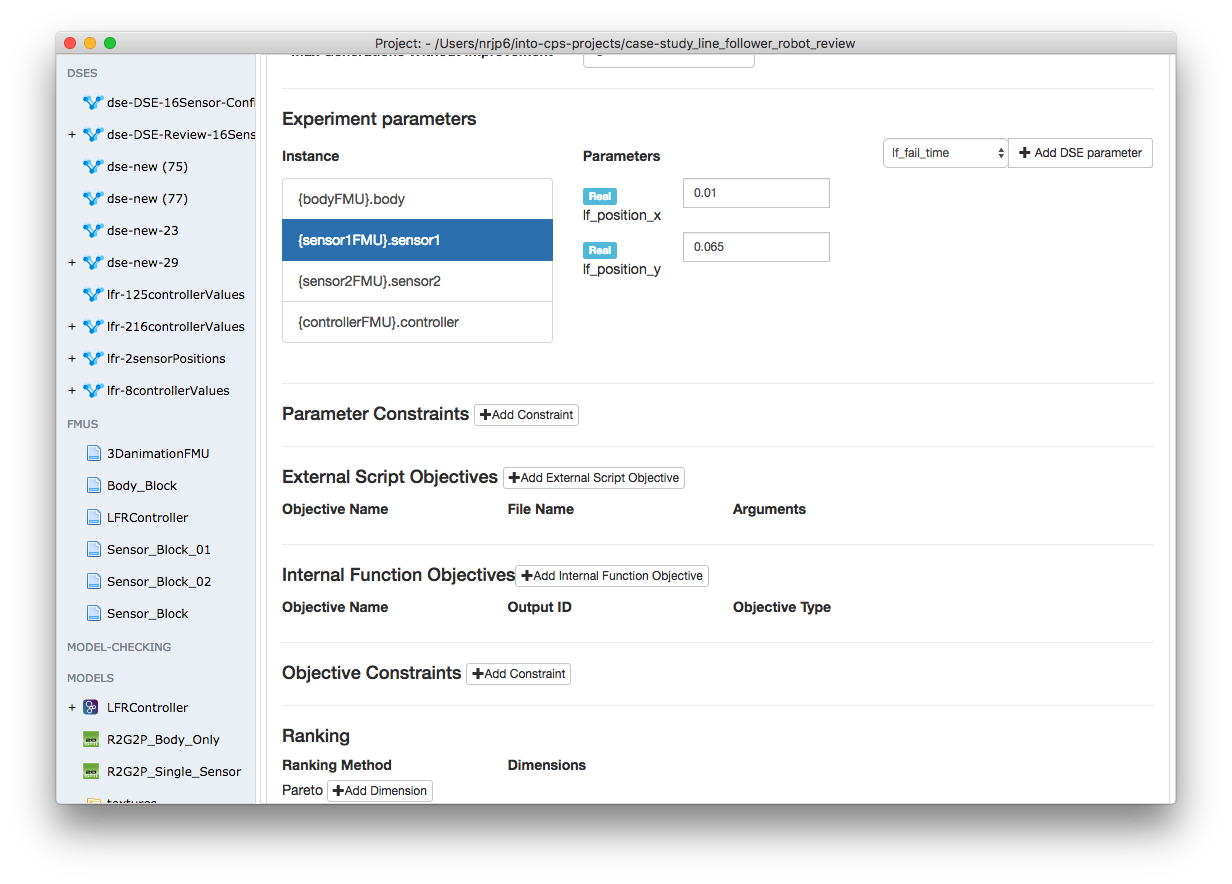
\includegraphics[width=0.9\textwidth]{figures/dse/app-param}
	\caption{Browsing the multi-model parameters.}\label{fig:dse:edit:app-param}
\end{figure}
%
%
%
\begin{figure}[ht]
	\centering
	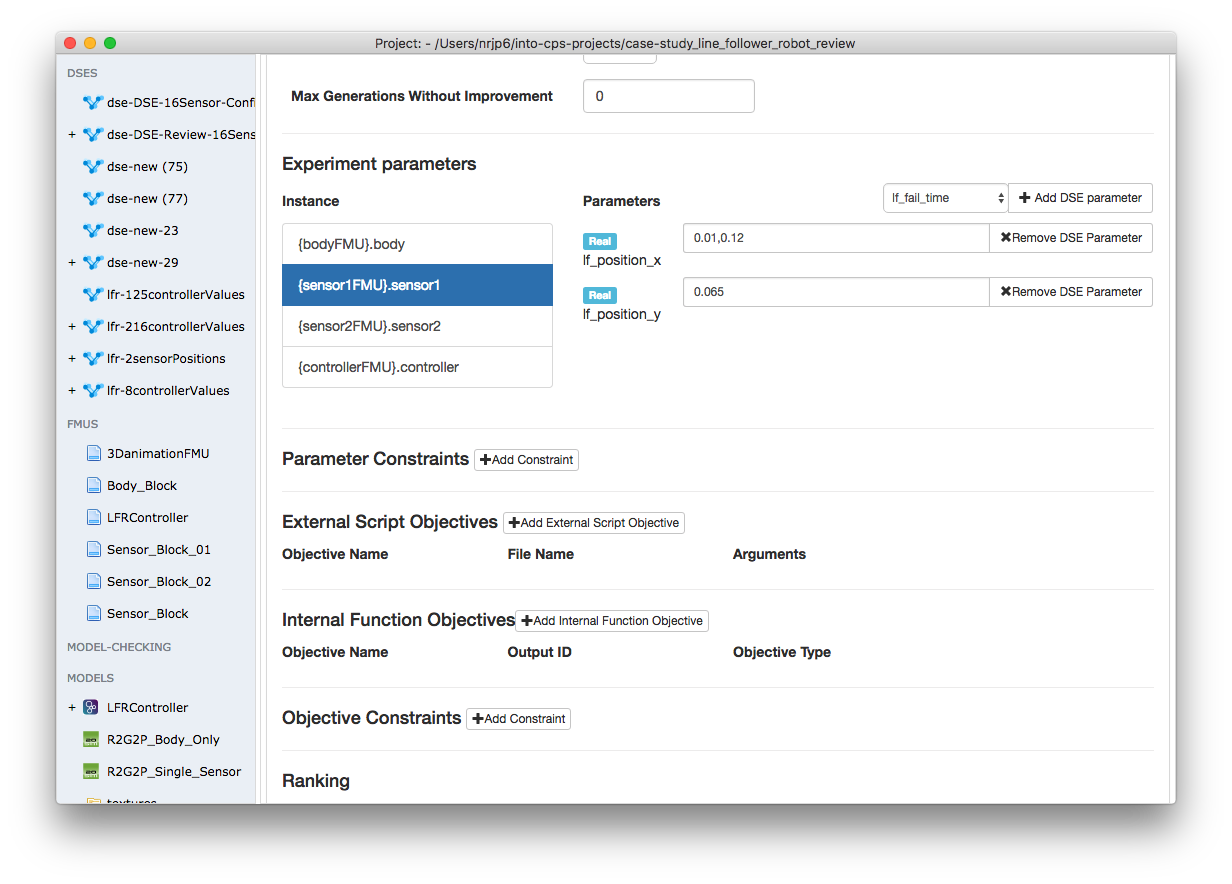
\includegraphics[width=0.9\textwidth]{figures/dse/app-param-edit}
	\caption{Editing parameters for DSE run.}\label{fig:dse:edit:app-param-edit}
\end{figure}
%
%
%

Parameters may be removed from the DSE configuration (they will not be removed from the multi-model) by clicking the \textit{Remove DSE Parameter} button -- see Figure~\ref{fig:dse:edit:app-param-remove}. Additional DSE parameters may be added by selecting the parameter name from the drop down and clicking the \textit{Add DSE Parameter} button -- see Figure~\ref{fig:dse:edit:app-param-add}.

\begin{figure}[ht]
	\centering
	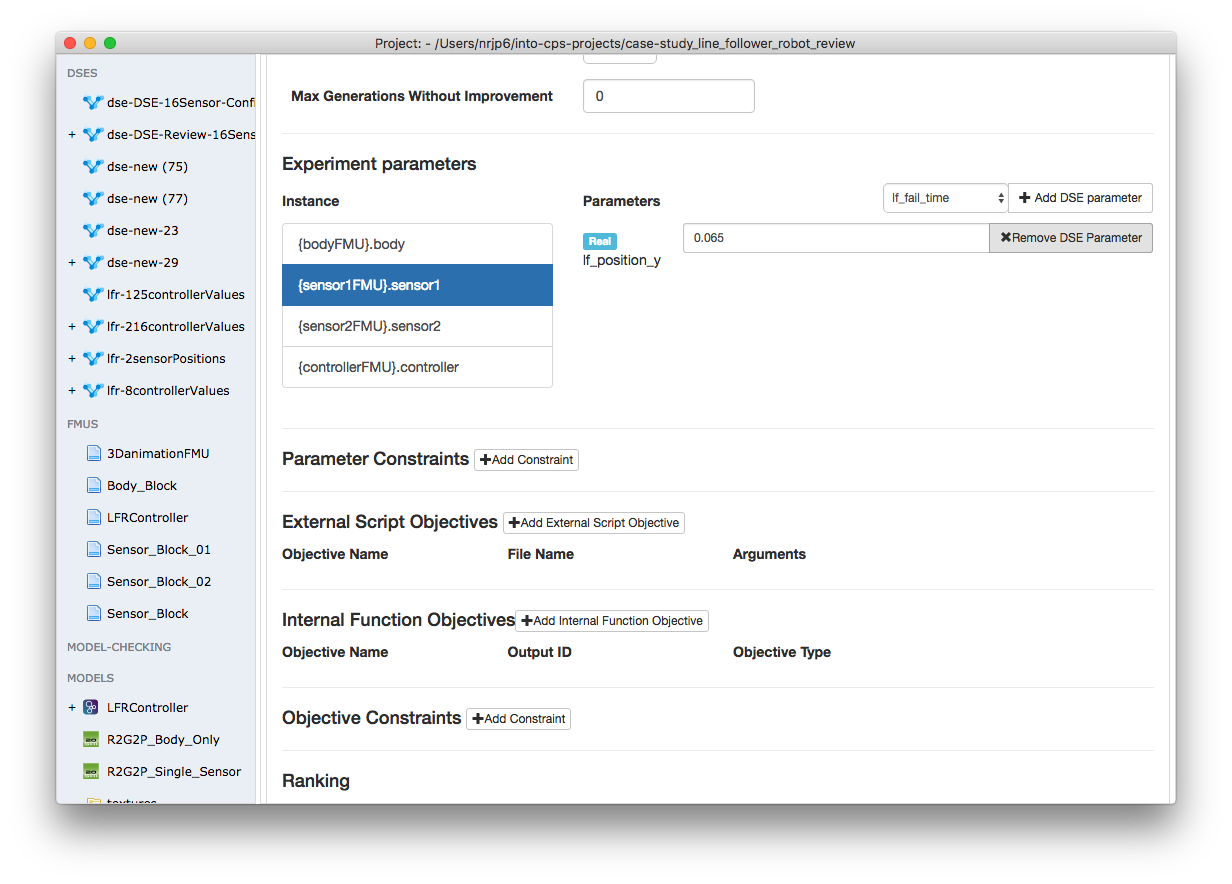
\includegraphics[width=0.9\textwidth]{figures/dse/app-param-remove}
	\caption{Removing a DSE parameter.}\label{fig:dse:edit:app-param-remove}
\end{figure}
%
%
%
\begin{figure}[ht]
	\centering
	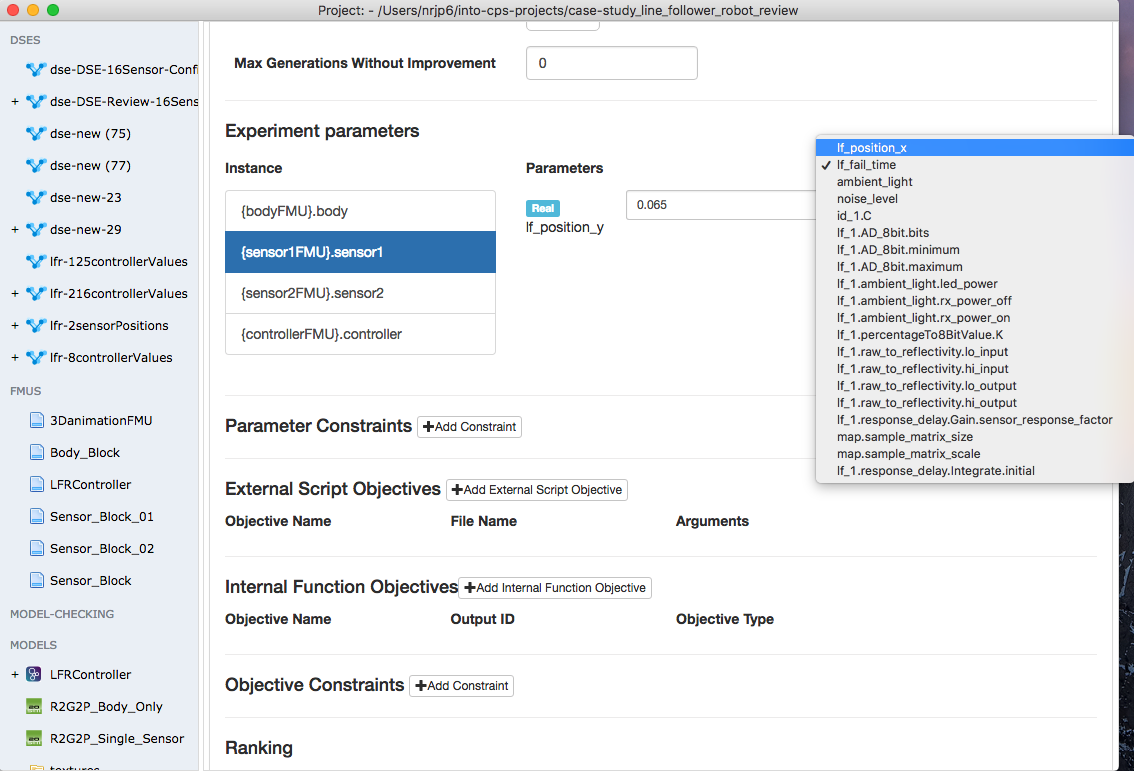
\includegraphics[width=0.9\textwidth]{figures/dse/app-param-add}
	\caption{Add a model parameter for DSE.}\label{fig:dse:edit:app-param-add}
\end{figure}
\clearpage
%
%
%

\subsubsection{Parameter Constraints}\label{sec:dse:app:parameterconstraints}

Clicking the \textit{Add Constraint} button in the Parameter Constraints section adds a text box where free text may be added, shown in Figure~\ref{fig:dse:edit:app-param-const}. The constraint must be defined according to the description in Section~\ref{sec:dse:edit:parameterconstraints}.

\begin{figure}[ht]
	\centering
	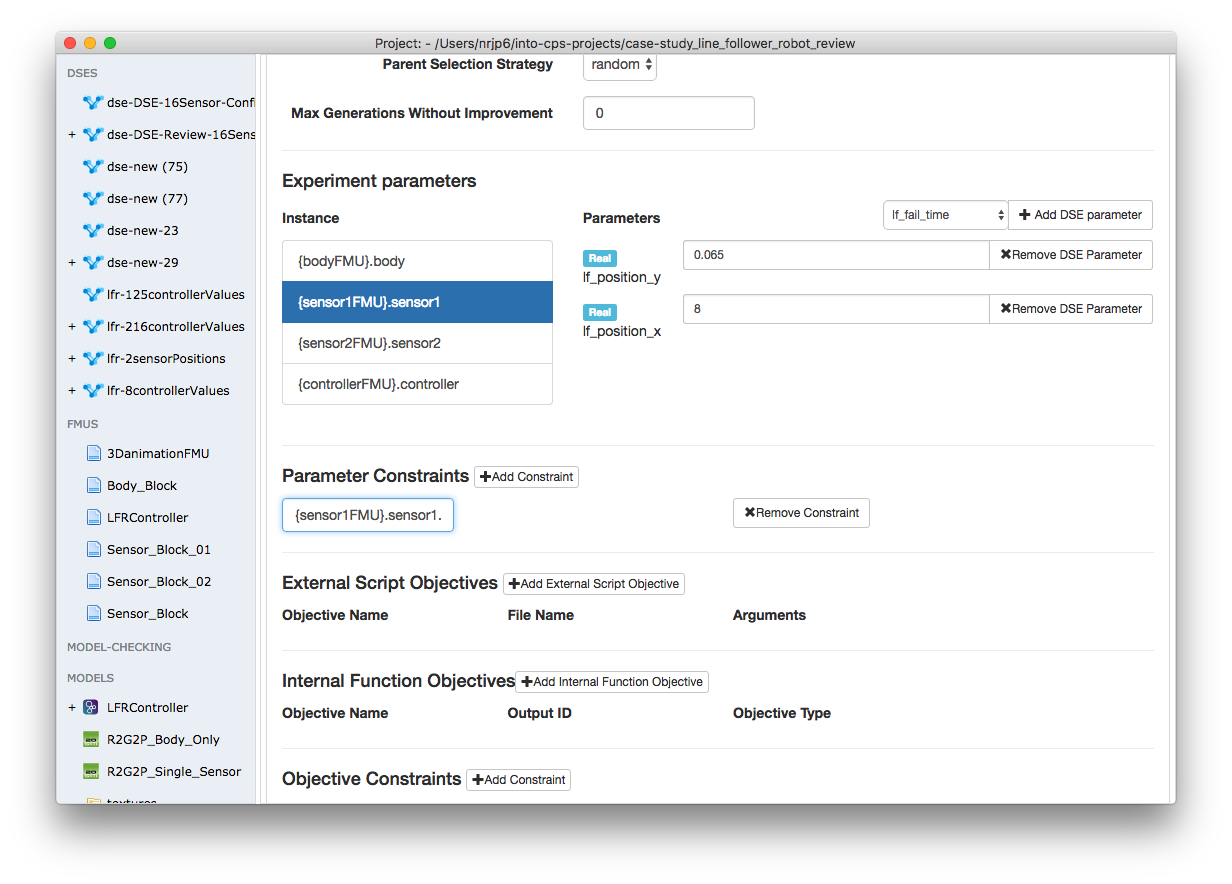
\includegraphics[width=0.9\textwidth]{figures/dse/app-param-const}
	\caption{Defining a parameter constraint.}\label{fig:dse:edit:app-param-const}
\end{figure}
%
%
%

\subsubsection{Objective Definitions: External Scripts}\label{sec:dse:app:objectivesexternal}

An external script can be added by clicking the \textit{Add External Script Objective} button. Two text boxes are added; first a name for the objective and the file name of the objective script. In Figure~\ref{fig:dse:edit:app-ext-new}, the new objective is given the name \textit{lapTime} and uses the \textit{lapTime.py} Python script. Note: external scripts must be included in the \textit{userMetricScripts} folder of the INTO-CPS project.

\begin{figure}[ht]
	\centering
	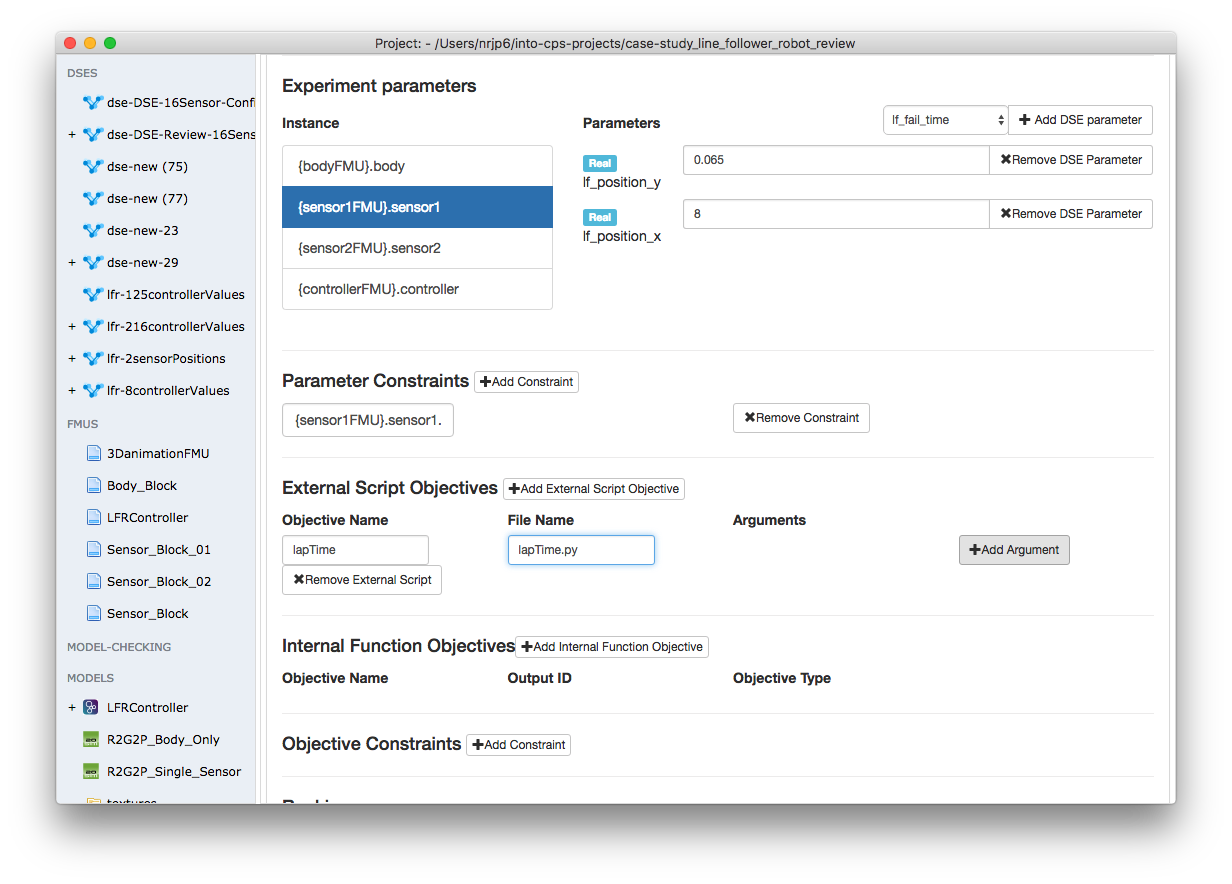
\includegraphics[width=0.9\textwidth]{figures/dse/app-ext-new}
	\caption{Adding a new external script.}\label{fig:dse:edit:app-ext-new}
\end{figure}
%
%
%

Once added, the required arguments must be given. Clicking the \textit{Add Argument} button adds several elements (shown in Figure~\ref{fig:dse:edit:app-ext-arg}) -- the first text box indicates the argument order;  the second drop down indicates the type of value, which is either a model output (refers to an output port of a constituent element of the multi-model), a simulation value (either \texttt{step-size} or \texttt{time}), or some constant; the third is the argument to pass to the script. The argument may be a user defined constant value, or one of the predefined values depending on the type selected. A complete definition is shown in Figure~\ref{fig:dse:edit:app-ext-done}. 

\begin{figure}[ht]
	\centering
	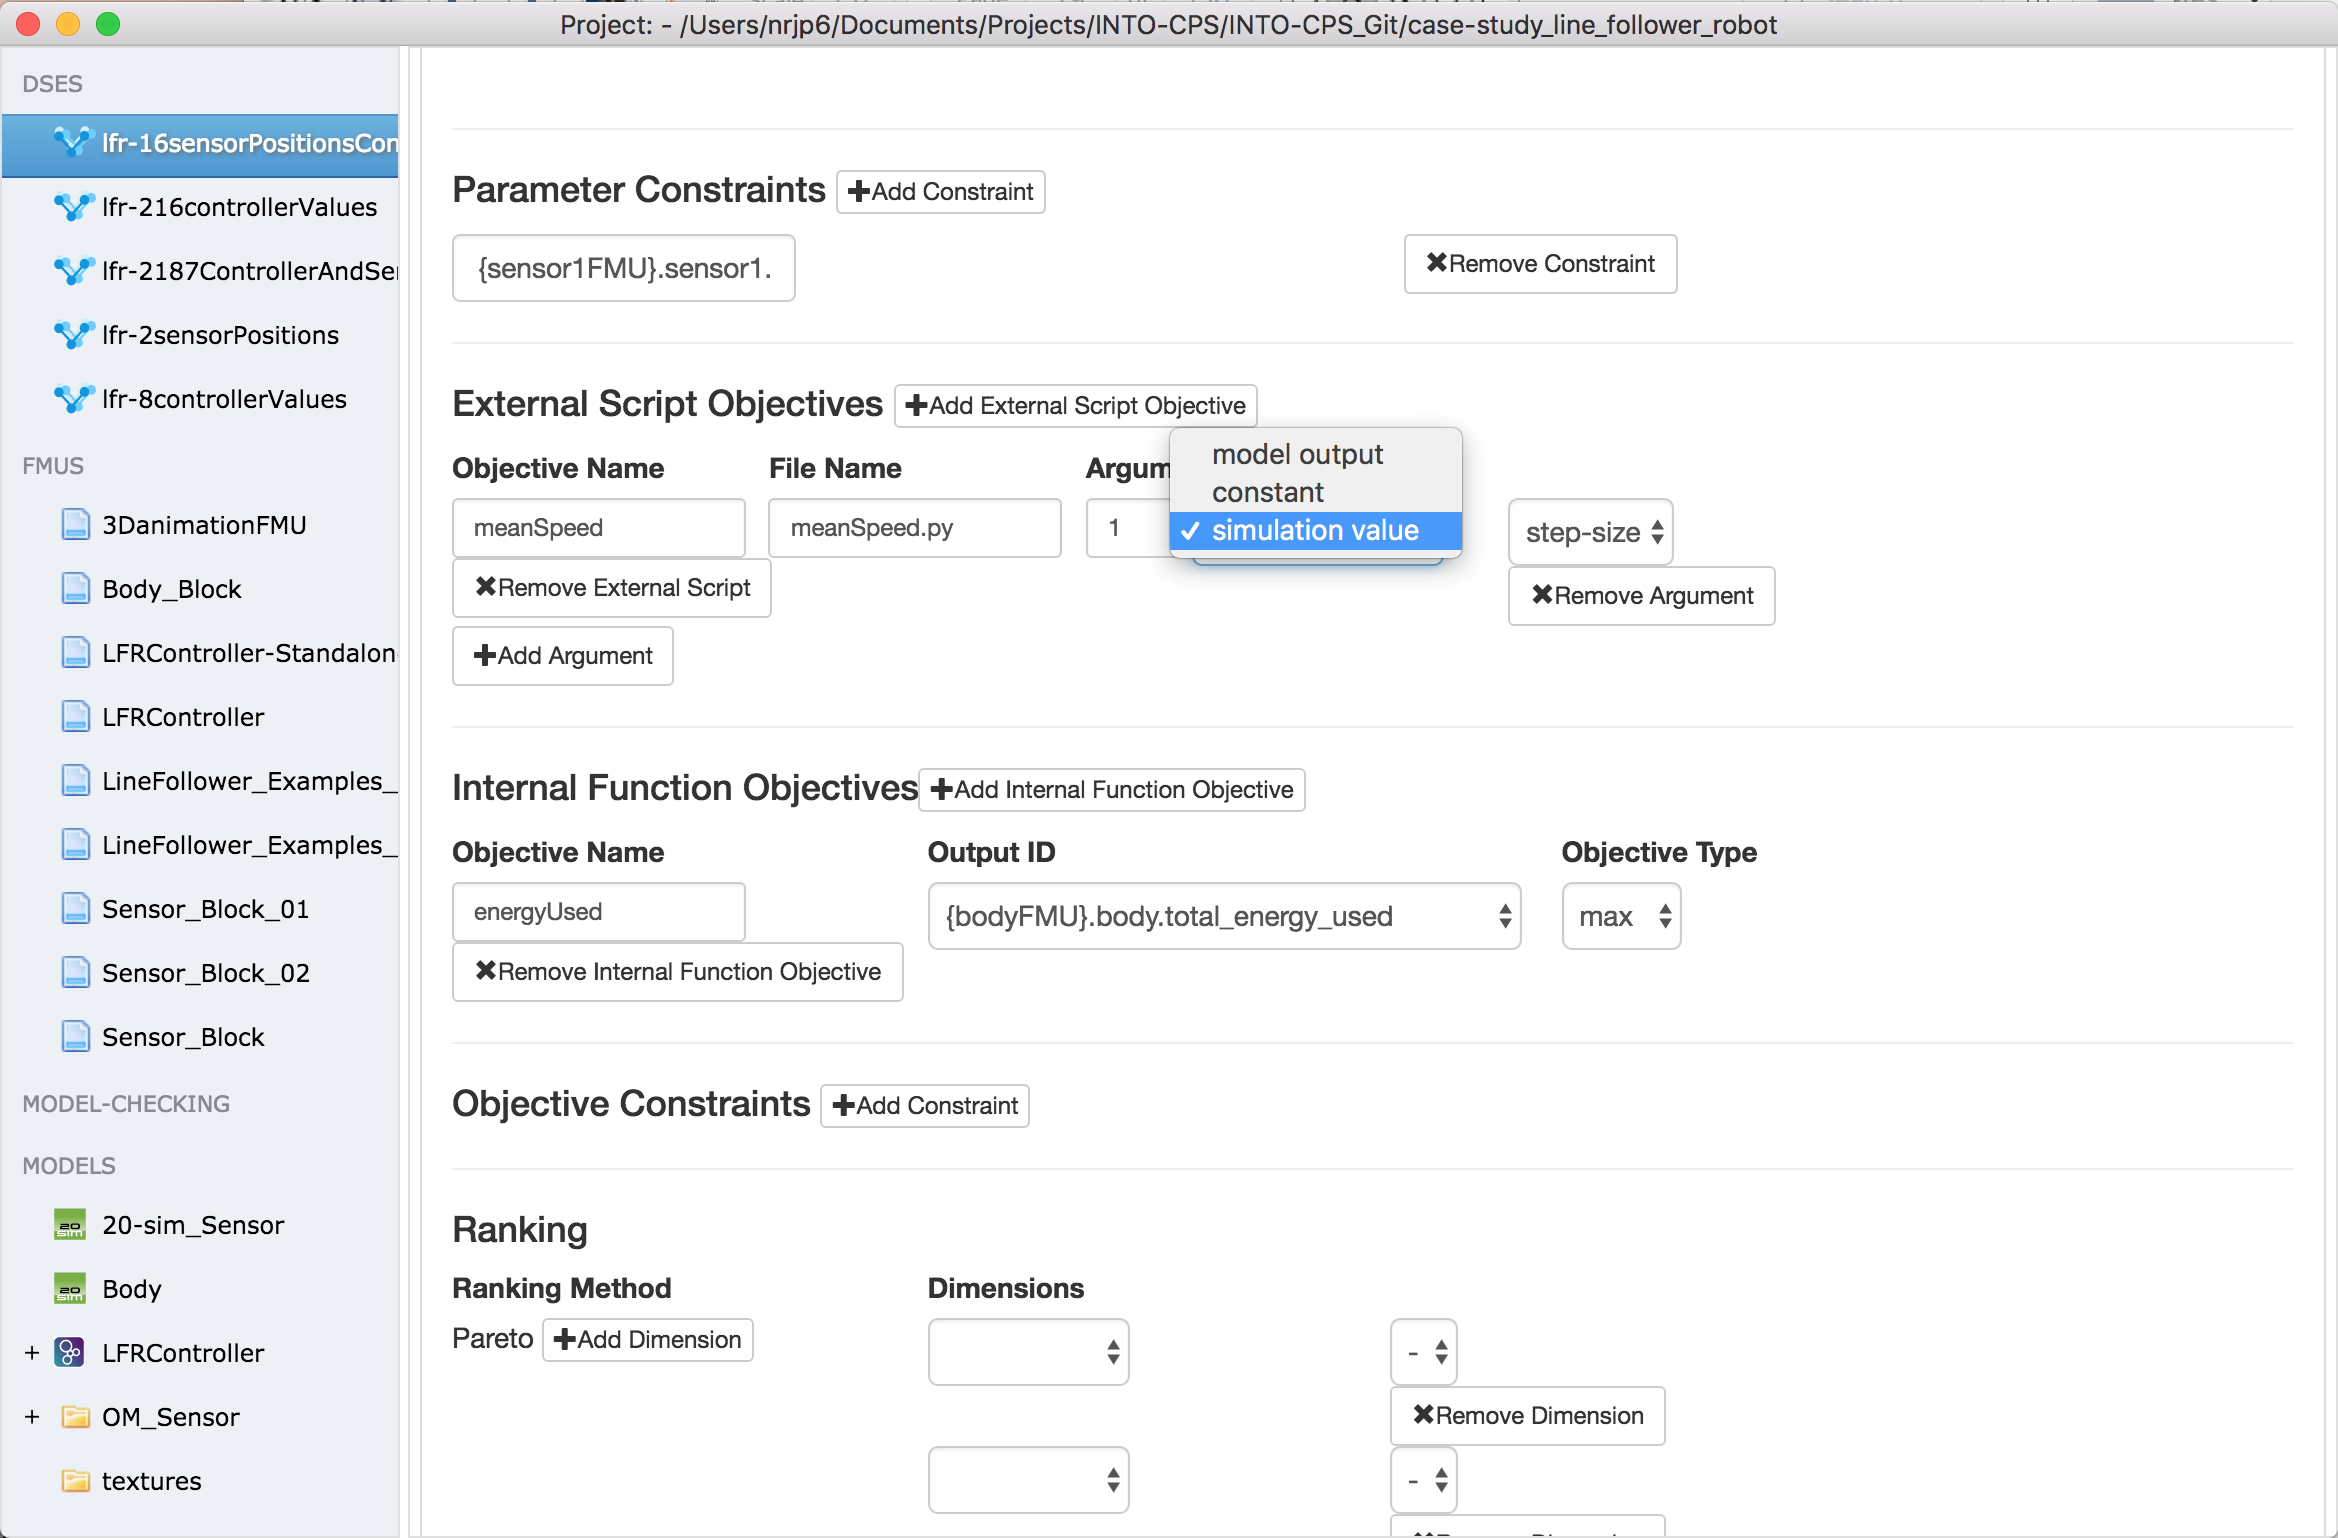
\includegraphics[width=0.9\textwidth]{figures/dse/app-ext-arg}
	\caption{Add argument to external script.}\label{fig:dse:edit:app-ext-arg}
\end{figure}
%
%
%
\begin{figure}[ht]
	\centering
	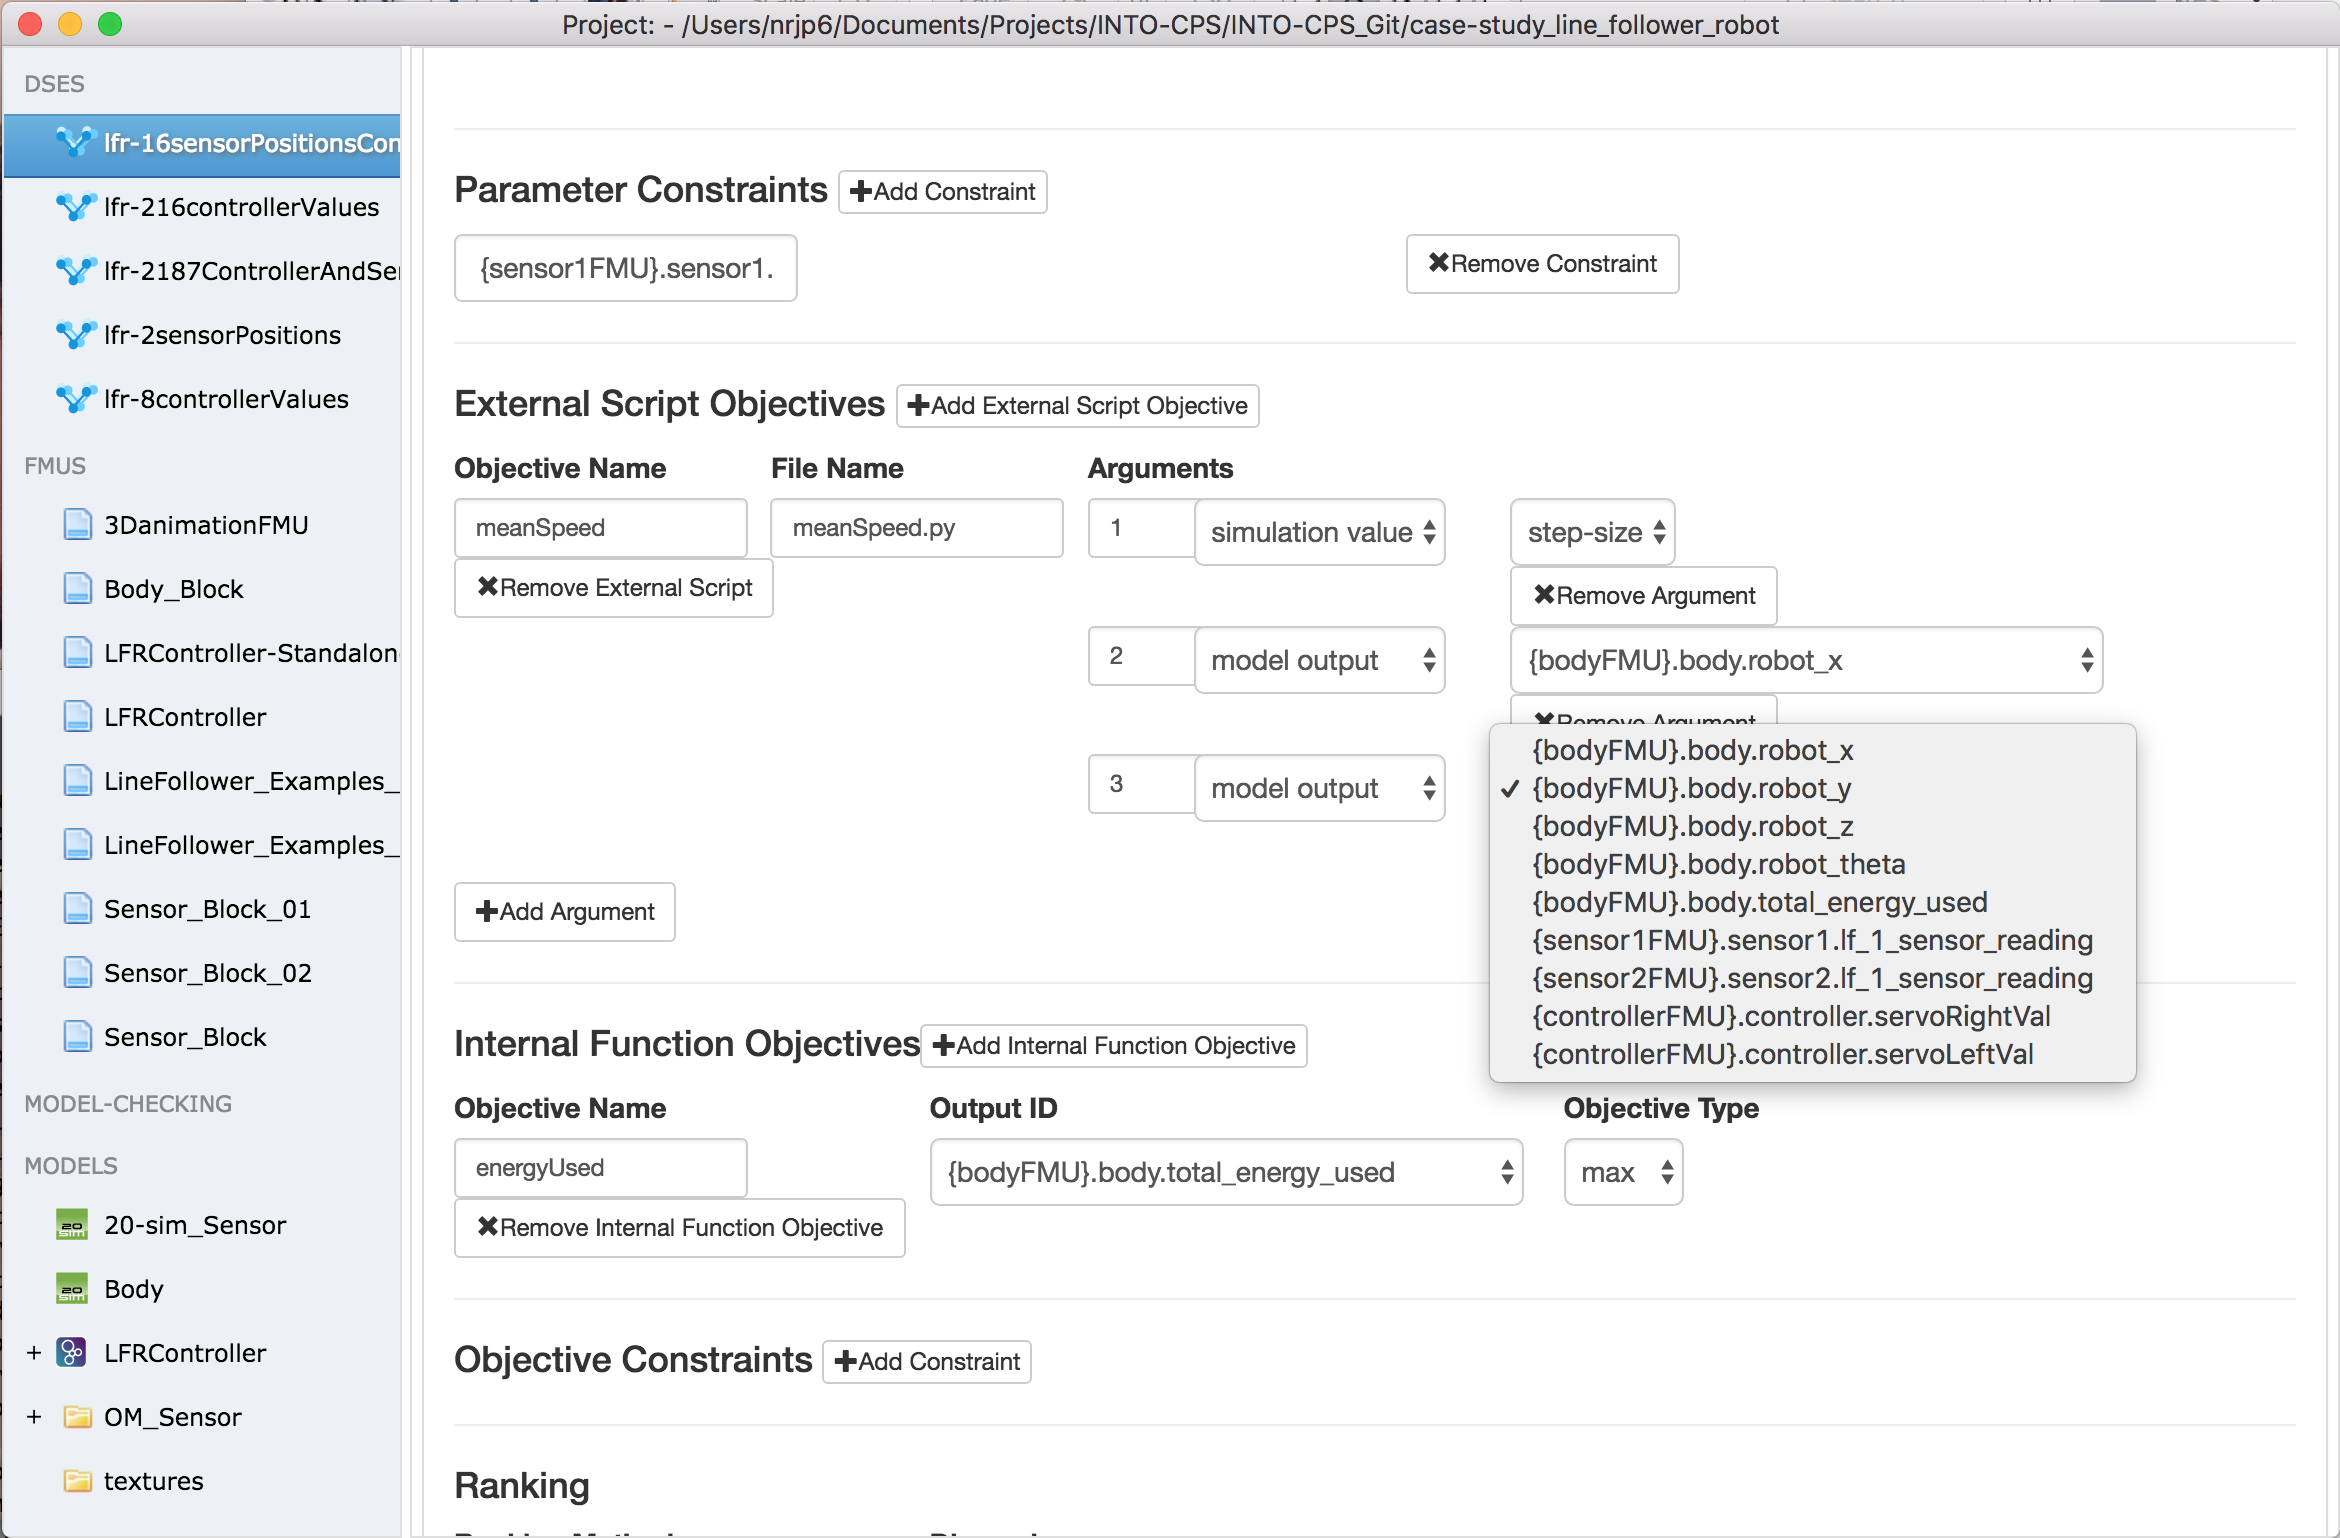
\includegraphics[width=0.9\textwidth]{figures/dse/app-ext-done}
	\caption{Complete external script.}\label{fig:dse:edit:app-ext-done}
\end{figure}
%
%
%


\subsubsection{Objective Definitions: Internal Functions}\label{sec:dse:app:objectivesinternal}

Internal functions are added by clicking the \textit{Add Internal Function Objective} button. This adds a text box to provide the name of the objective, a drop down to specify which model output to use (this refers to an output port of a constituent element of the multi-model) and a drop down to select the type of function. Currently three exist: \textit{max}, \textit{min} and \textit{mean}. This is shown in Figure~\ref{fig:dse:edit:app-internal}.

\begin{figure}[ht]
	\centering
	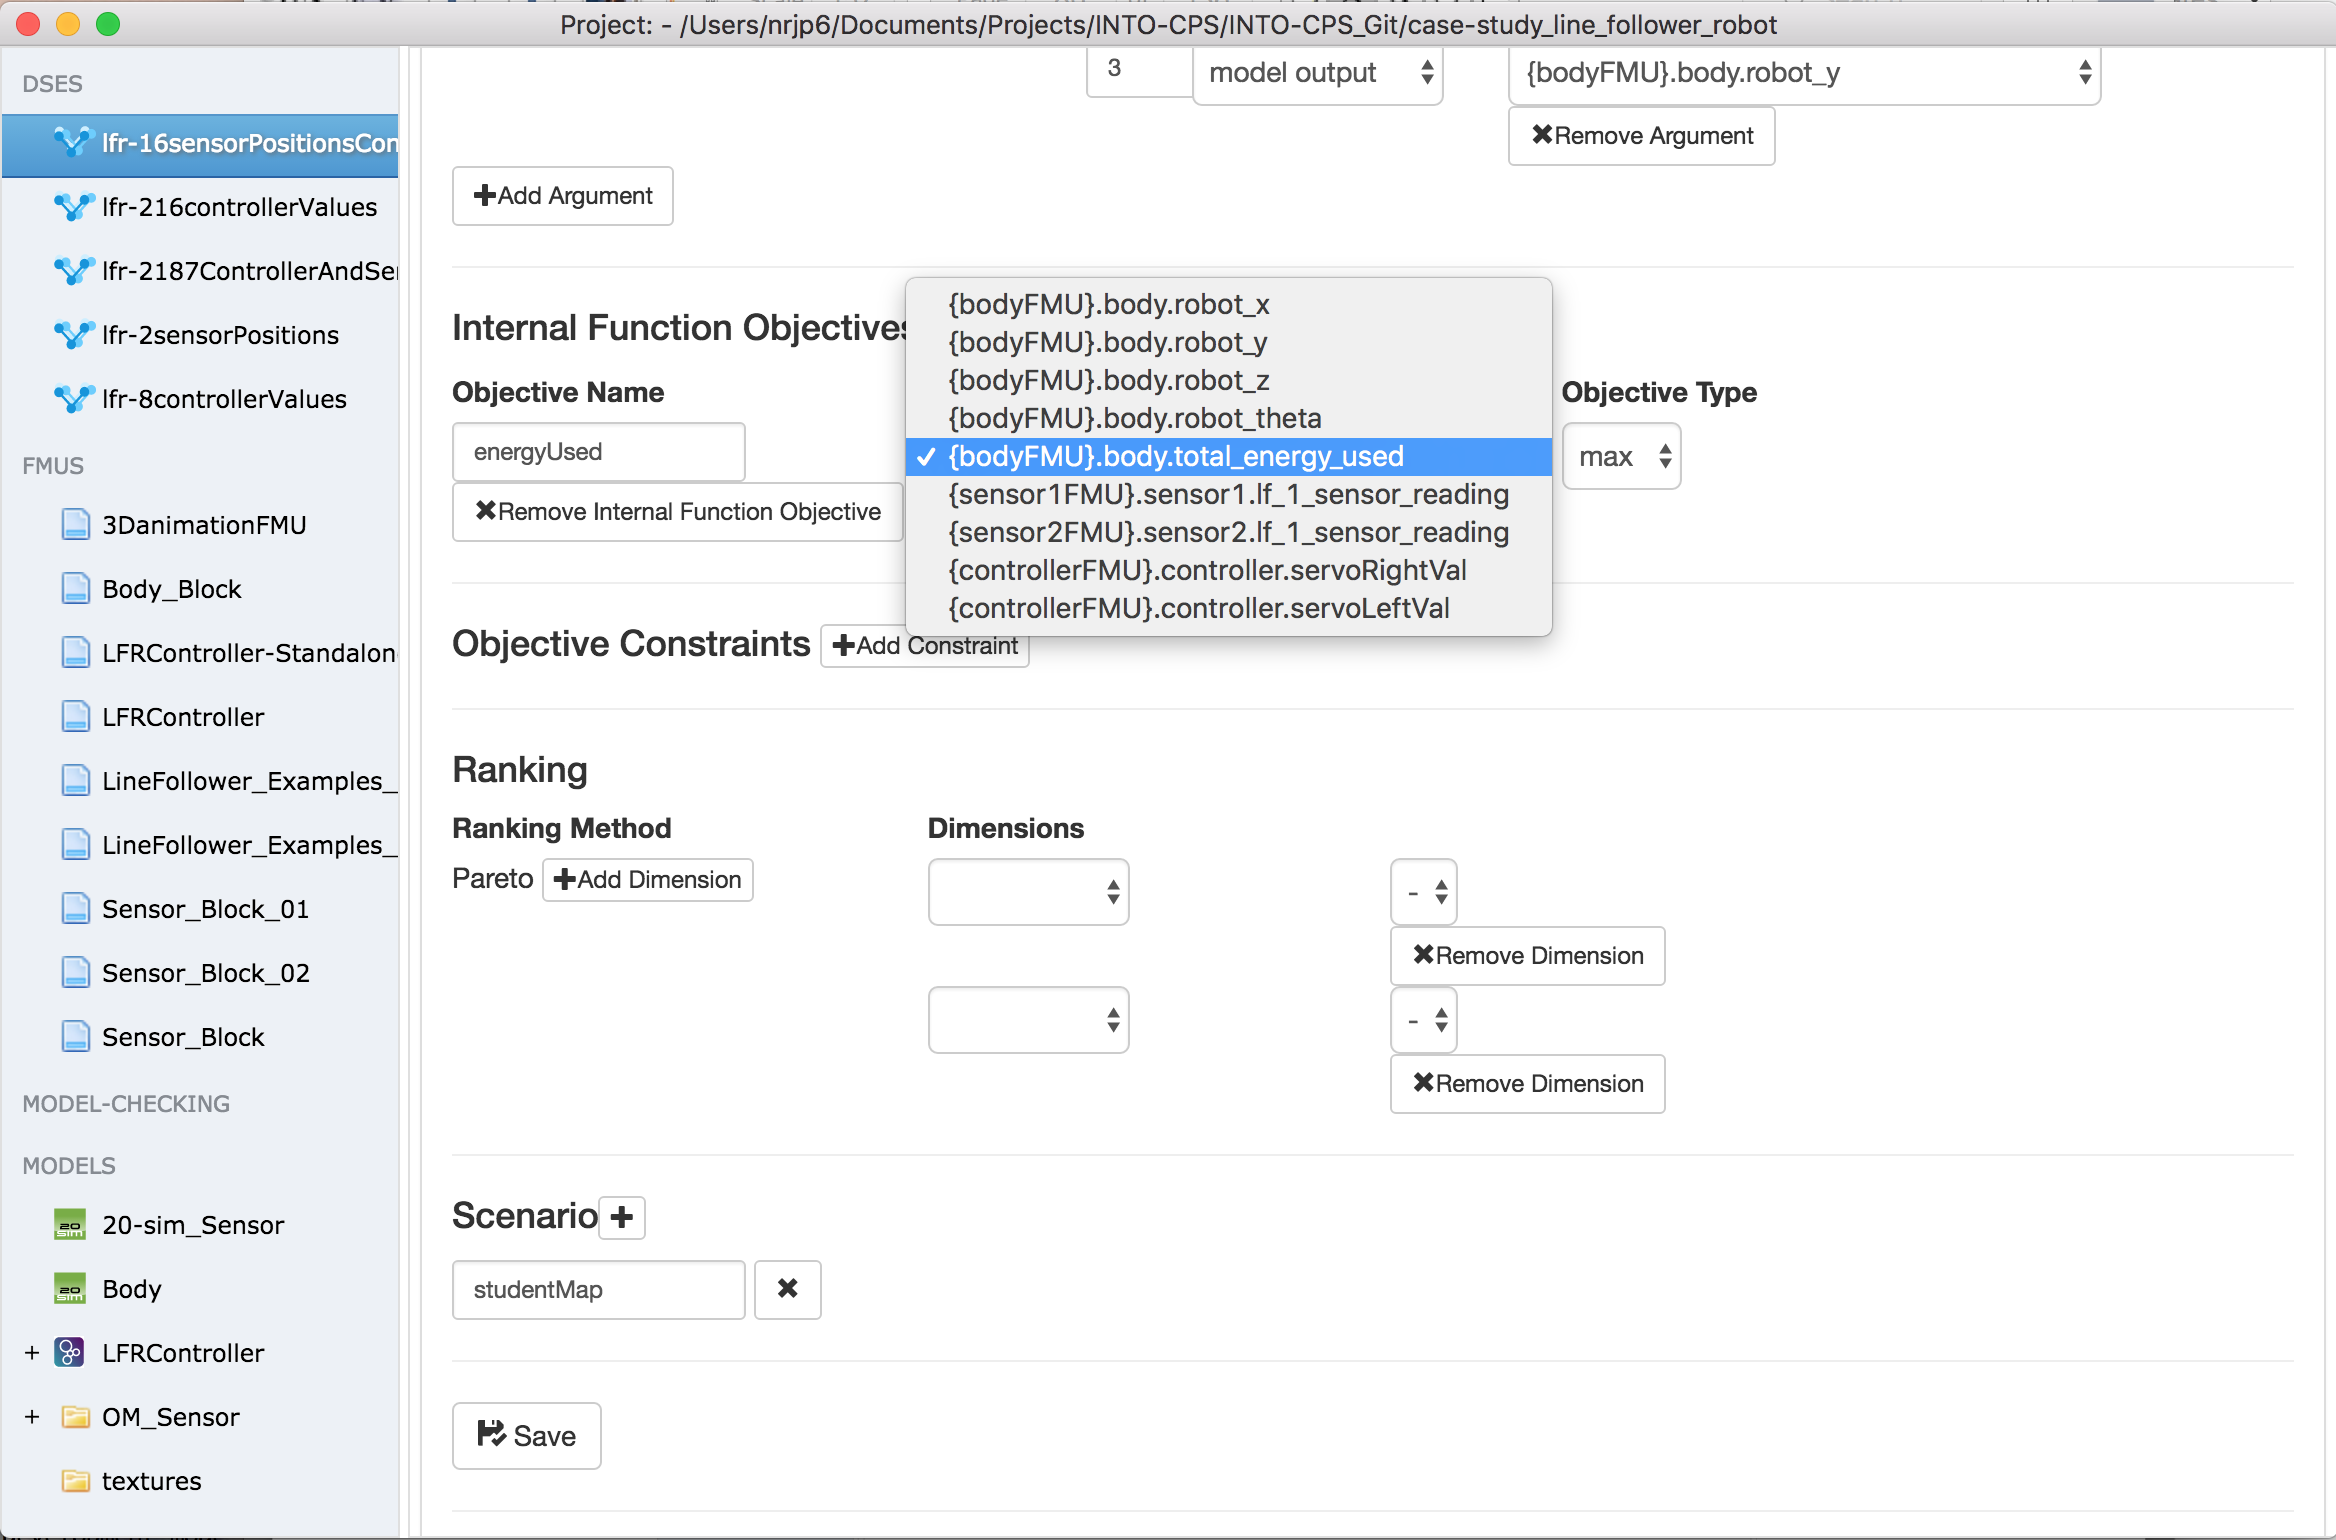
\includegraphics[width=0.9\textwidth]{figures/dse/app-internal}
	\caption{Defining an internal function.}\label{fig:dse:edit:app-internal}
\end{figure}
%
%
%
\subsubsection{Objective Constraints}\label{sec:dse:app:objectiveconstraint}
Objective constraints are similar to parameter constraints. A constraint is added by clicking the \textit{Add Constraint} button in the Objective Constraints section.  This adds a text box where free text may be added, shown in Figure~\ref{fig:dse:edit:app-obj-const}.  The constraint must be expressed in valid Python code.
%
%
%
\begin{figure}[ht]
	\centering
	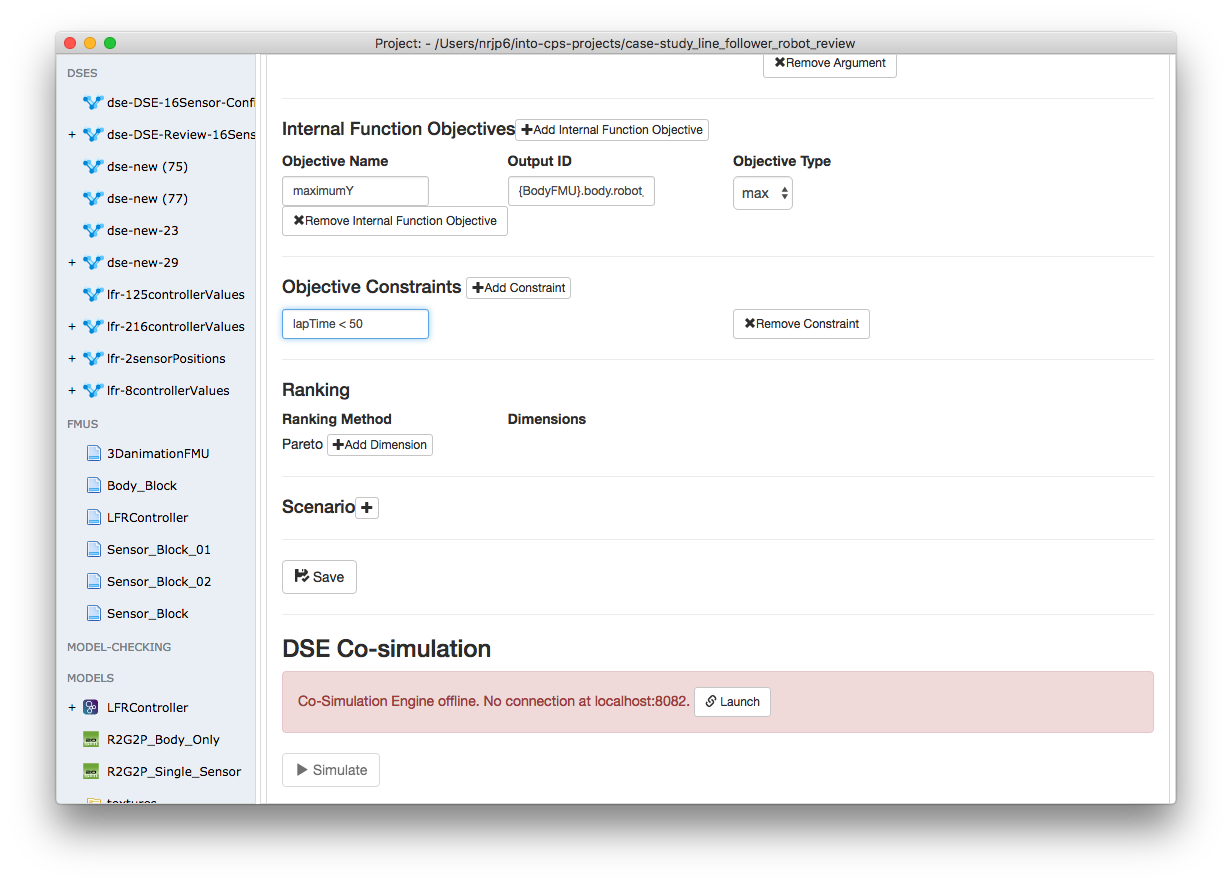
\includegraphics[width=0.9\textwidth]{figures/dse/app-obj-const}
	\caption{Defining an objective constraint.}\label{fig:dse:edit:app-obj-const}
\end{figure}
%
%
%
\subsubsection{Ranking}\label{sec:dse:app:ranking}
At present, DSE uses only 2-way Pareto rankings. As such, a maximum of two dimensions may be added by clicking the \textit{Add Dimension} button. When clicked, the user may select one of the defined objectives and a direction -- either $+$ or $-$. This is shown in Figure~\ref{fig:dse:edit:app-ranking-dimension}.
%
%
%
\begin{figure}[ht]
	\centering
	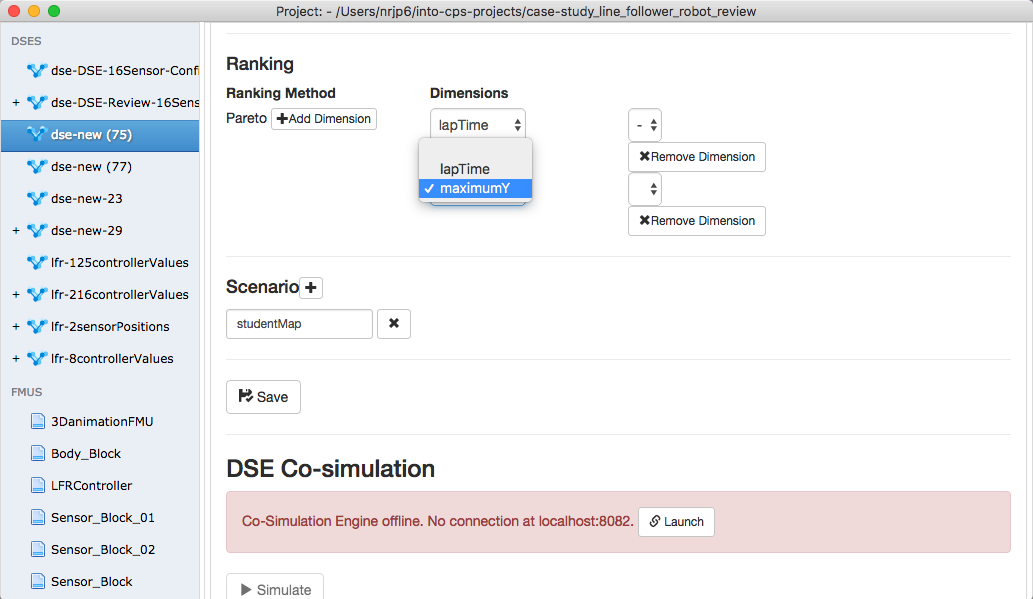
\includegraphics[width=0.9\textwidth]{figures/dse/app-ranking-dimension}
	\caption{Defining the Pareto ranking.}\label{fig:dse:edit:app-ranking-dimension}
\end{figure}
%
%
%
\subsubsection{Scenario List}\label{sec:dse:app:scenarios}
The support for scenarios is currently limited. At present the user may define a collection of named scenarios, which are passed to all external scripts (the external scripts need not use this). This is shown in Figure~\ref{fig:dse:edit:app-scen}.
%
\begin{figure}[ht]
	\centering
	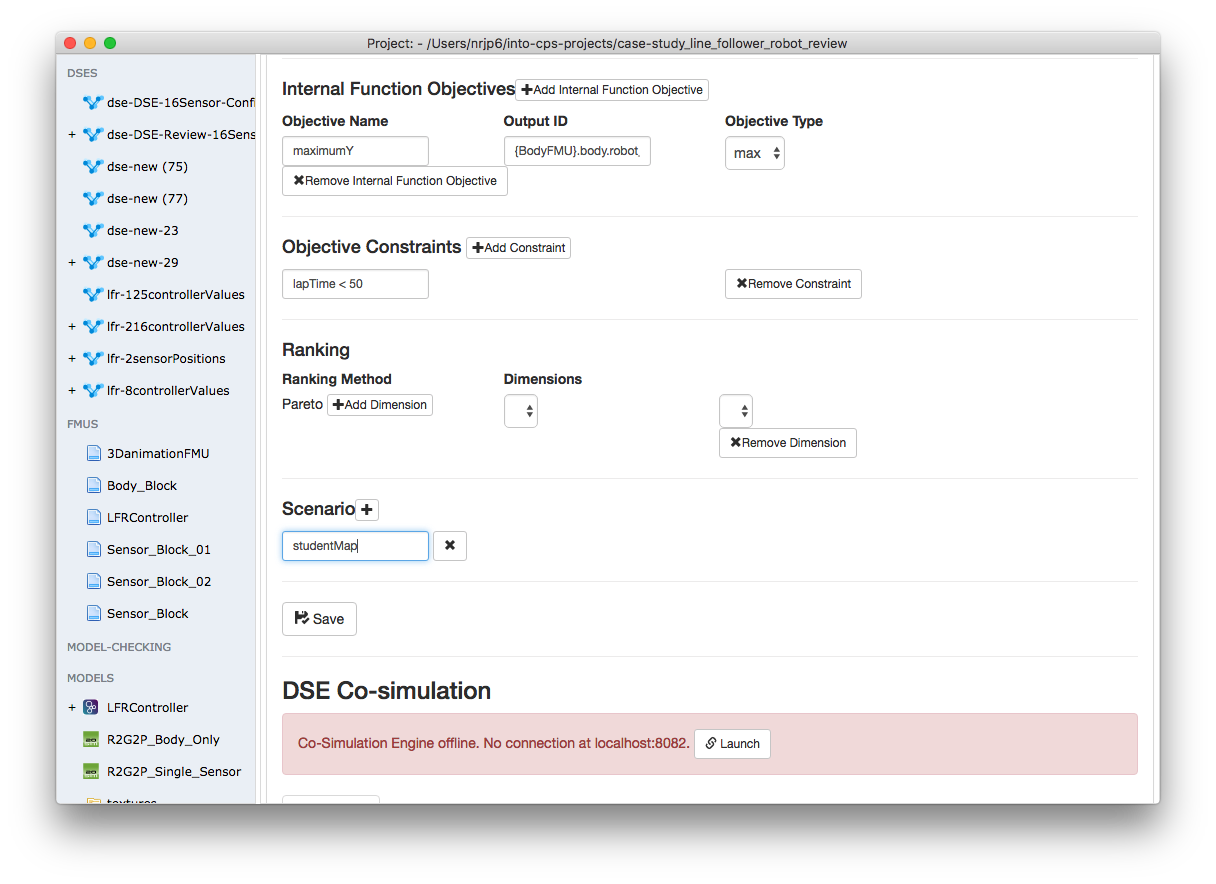
\includegraphics[width=\textwidth]{figures/dse/app-scen}
	\caption{Adding a DSE scenario.}\label{fig:dse:edit:app-scen}
\end{figure}
%
%
%
\subsubsection{Saving the Configuration}\label{sec:dse:app:save}

When the configuration editing is finished, it may be saved by clicking the \textit{Save} button at the top or bottom of the configuration description, as in Figure~\ref{fig:dse:edit:app-save}. Note this will overwrite the previous version of the json configuration file -- any non-DSE tags will be lost.

\begin{figure}[ht]
	\centering
	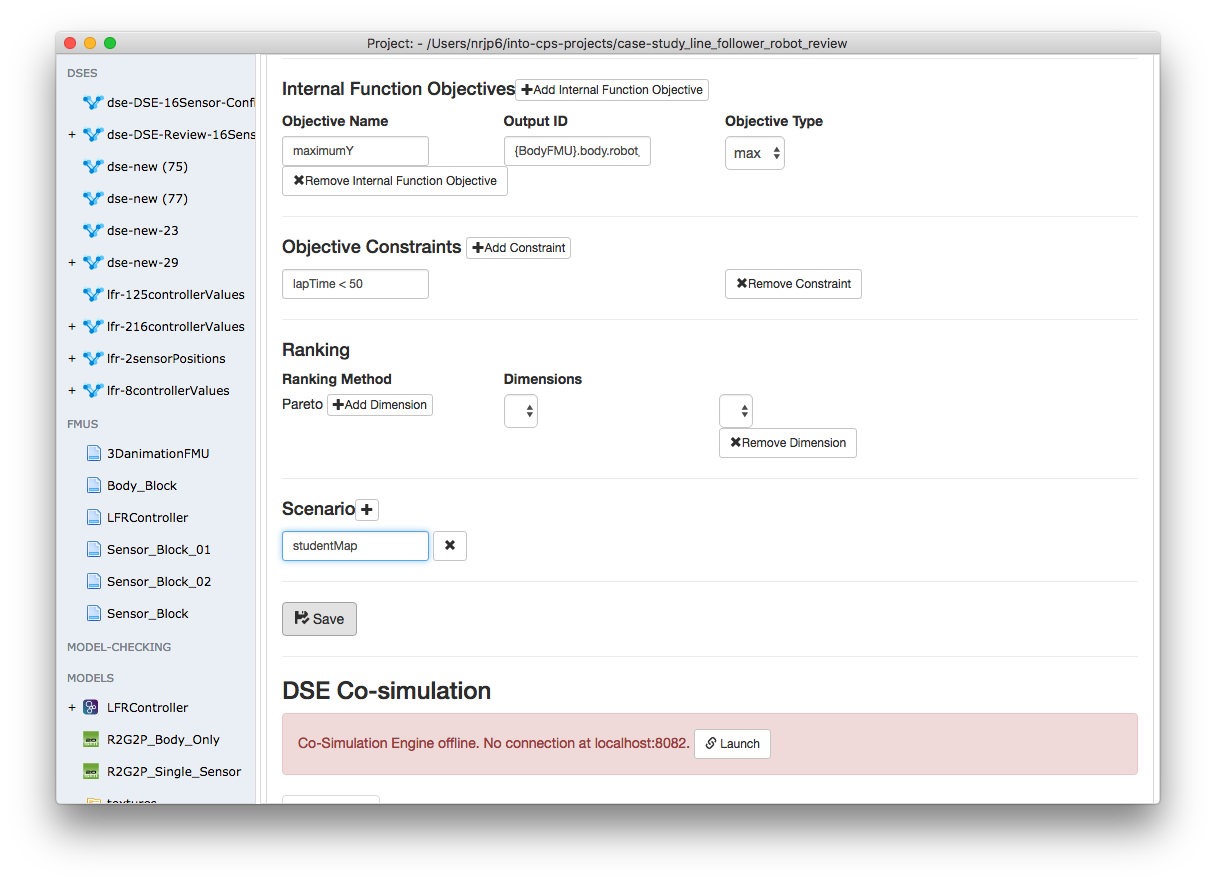
\includegraphics[width=\textwidth]{figures/dse/app-save}
	\caption{Save DSE configuration.}\label{fig:dse:edit:app-save}
\end{figure}
%
%
%
\subsubsection{Manual Configuration Creation}\label{sec:dse:edit:manual}
The recommended procedure for creating a new configuration is to make a copy of an existing one and then to edit the required sections.  The individual configurations are located in their own folders within the \textit{Design Space Exploration} folder of the \intoapp{} project directory, such as the pilot study with the line following robot ``LFR-2SensorPositions'' configuration shown in Figure~\ref{fig:dse:edit:location} (see \cite{INTOCPSD3.5}).  Using your OS's file browser, create a new folder under \textit{DSEs} and then copy in and rename a DSE configuration.  The names of the new folder and configuration folder can be chosen at will, but the configuration file must have the extension \texttt{.dse.json} .  
%
%
%
\begin{figure}[ht]
	\centering
	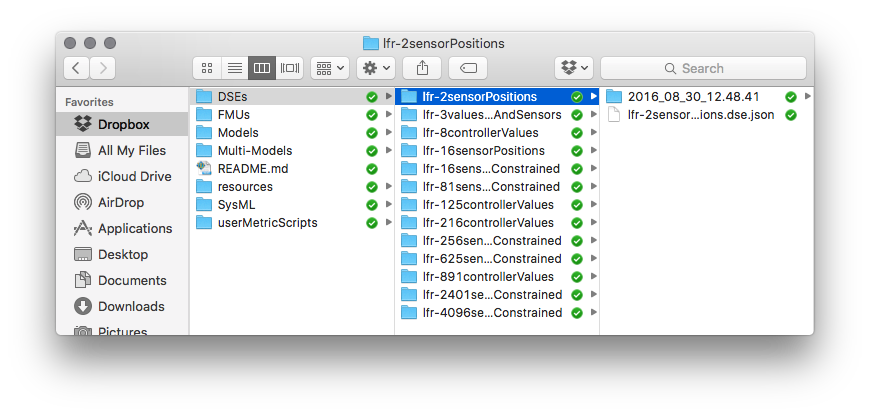
\includegraphics[width=\textwidth]{figures/dse/config-location}
	\caption{Location of DSE configurations.}\label{fig:dse:edit:location}
\end{figure}
%
%
%
\subsubsection{Algorithm}\label{sec:dse:edit:algorithm}

The algorithm section dictates the DSE search algorithm to employ in a DSE. There are two types (although if no algorithm is defined, it is assumed to be an exhaustive search):
%
%
\begin{description}
	\item [Exhaustive] No further values are required.
	\item[Genetic] The genetic approach requires several additional values; initialPopulation (number); initialPopulationDistribution (currently only ``random'' is supported); mutationProbablity (number -- 0-100); parentSelectionStrategy (currently only ``random'' is supported); and maxGenerationsWithoutImprovement (number).
\end{description}
%

An example is given in Figure~\ref{fig:dse:edit:algorithm}.

\begin{figure}[ht]
	\centering
	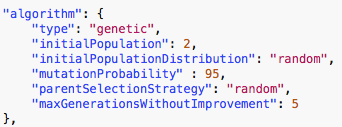
\includegraphics[scale=0.55]{figures/dse/config-algorithm}
	\caption{Example genetic algorithm.}\label{fig:dse:edit:algorithm}
\end{figure}
%
%
\subsubsection{Parameters}\label{sec:dse:edit:parameters}
%Compare \texttt{\string{\string}} to \verb|{}| and \texttt{\{\}}
The parameters section is used to define a list of values for each parameter to be explored.  Figure~\ref{fig:dse:edit:parameters} shows the definition of four parameters, each with two values. If a parameter is included in the DSE configuration file, then it must have at least one value defined.  The order of the values in the list is not important.  If a parameter that is to be explored is not in the list, its ID may be found in the three ways listed below.
%
%
%
\begin{enumerate}
	\item If the parameter is listed in the multi-model configuration, then copy it from there.
	\item If the parameter is not in the multi-model parameters list then its name may be found by examining the model description file in the associated FMU.  In this case it will be necessary to prepend the parameter ID with the ID for the FMU and the instance ID of the FMU, for example in ``\texttt{\string{sensor1FMU\string}.sensor1.lf\_position\_x}''.
	%
	%
	%
	\begin{itemize}
	\item  the ID of the FMU is \texttt{\string{sensor1FMU\string}}.
	\item  the instance ID of the FMU in the multi-model is \texttt{sensor1}.
	\item  the parameter ID is \texttt{lf\_position\_x}.
	\end{itemize}
	%
	%
	%
	\item The IDs for each parameter may also be found on the Architecture Structure Diagram in the SysML models of the system.  The  full name for use in the multi-model may then be constructed as above.
\end{enumerate}
%
%
%
\begin{figure}[ht]
	\centering
	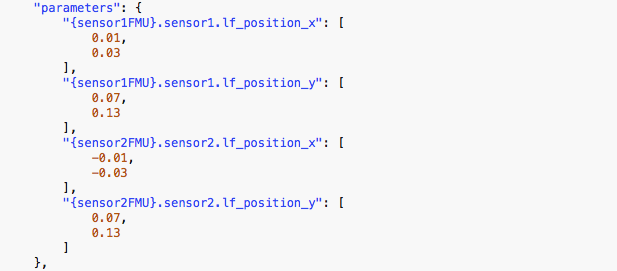
\includegraphics[scale=0.55]{figures/dse/config-parameters}
	\caption{Example parameter definitions.}\label{fig:dse:edit:parameters}
\end{figure}
%
%
%
\subsubsection{Parameter Constraints}\label{sec:dse:edit:parameterconstraints}

Figure \ref{fig:dse:edit:parameterconstraints} shows two constraints defined for the line follower DSE experiment that ensure only symmetrical designs are allowed.  The first constraint ensures the y co-ordinates of both sensors are the same, while the second constraint ensures that the x co-ordinate of the left sensor is the same, but negated as the x co-ordinate of the right sensor.  Note that the names used when defining such constraints have the same \texttt{FMU\_ID.\@instance\_ID.\@parameter\_ID} format as used when defining a parameter range (see Section~\ref{sec:dse:edit:parameters})

Since the constraints are processed using the Python \texttt{eval} function, any boolean expression compatible with this may be used here.
%
%
%
\begin{figure}[ht]
	\centering
	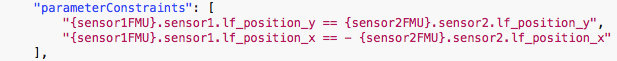
\includegraphics[scale=0.55]{figures/dse/config-parameterconstraints}
	\caption{Example parameter constraints.}\label{fig:dse:edit:parameterconstraints}
\end{figure}
%
%
%

%
%
%
%\begin{figure}[ht]
%	\centering
%	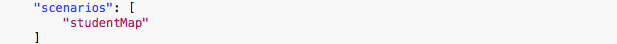
\includegraphics[scale=0.55]{figures/dse/config-scenarios}
%	\caption{Example scenario definition.}\label{fig:dse:edit:scenarios}
%\end{figure}
%
%
%
\subsubsection{Objective Definitions: Internal}\label{sec:dse:edit:objectivesinternal}


Defining an internal objective requires three pieces of information:
%
%
%
\begin{description}
	\item[name] This is the name that the objective value will be stored under in the objectives file.
	\item[type] This selects the function to be applied.  The key \texttt{objectiveType} is used in the DSE configuration file.
	\item[variable] This defines the variable to which the function is to be applied.  The key \texttt{columnID} is used to denote this parameter in the DSE configuration file.
\end{description}
%
%
%
Figure~\ref{fig:dse:edit:objectivesinternal} shows the definition of an objective named \texttt{energy\-Consumed}, which records the maximum value of the variable \newline \texttt{\string{bodyFMU\string}.body.total\_energy\_used}.  This objective is recorded and may be used later, primarily for the purpose of ranking designs, but it could also be used for any other analysis required.
%
%
%
\begin{figure}
	\centering
	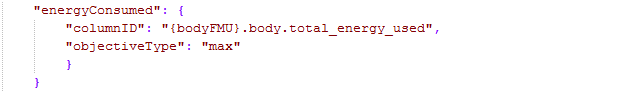
\includegraphics[width=0.9\textwidth]{figures/dse/config-objectivesinternal}
	\caption{Definition of an internal objective.}\label{fig:dse:edit:objectivesinternal}
\end{figure}
%
%
%
\subsubsection{Objective Definitions: External Scripts}\label{sec:dse:edit:objectivesexternal}

Using external scripts in a configuration requires three parts; a name for the objective, the file name of the script and a list of arguments to pass.  The name given to the objective allows it to be referenced in the objectives constraints and ranking sections of the DSE configuration.  The file name tells the DSE scripts which script to launch and the arguments define additional data (over the standard three arguments described earlier) that the script needs, such as the names of data it needs or constant values.

In Figure \ref{fig:dse:edit:objectivesexternal-ttwt} we find the definition of the external analysis used in the Three Water Tank example.  There are two analyses defined, the first is named ``cumulativeDeviation'' and the second is ``vCount''.  In each there are two parameters defined:  ``scriptFile'' contains the file name of the script file to run in each case, while ``scriptParameters'' contains the list of additional arguments each needs.  
%
%
%
\begin{figure}[ht]
	\centering
	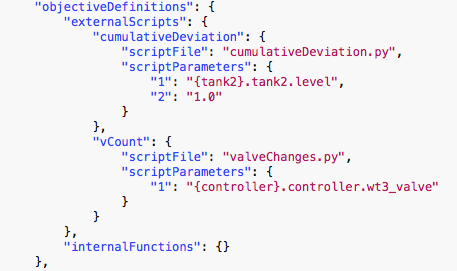
\includegraphics[scale=0.55]{figures/dse/config-objectivesexternal-ttwt}
	\caption{Definition of the external analysis functions for the Three Water Tank model.}\label{fig:dse:edit:objectivesexternal-ttwt}
\end{figure}
%
%
%

The purpose of both internal and external analysis functions is to populate the \texttt{objectives.json} file with values that characterise the performance of the designs being explored.  Figure \ref{fig:dse:edit:objectivejson} shows an example objectives file generated during a DSE of the Three Water Tank example.  There is an instance of the objectives file created for each simulation in DSE, its primary use being to inform the ranking of designs, but it may be used for any other analysis a user wishes to define.
%
%
%
\begin{figure}[ht]
	\centering
	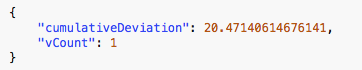
\includegraphics[scale=0.55]{figures/dse/objectivejson}
	\caption{Contents of \texttt{objectives.json} file for a single simulation of the Three Water Tank model.}\label{fig:dse:edit:objectivejson}
\end{figure}
%
%
%
\subsubsection{Ranking}\label{sec:dse:edit:ranking}

Figure~\ref{fig:dse:edit:ranking} shows an example of a ranking definition from the line following robot example.  Here the user has specified that the lap time and mean cross track error objectives will be used for ranking.  The use of '-' after each indicates that the aim is to minimise both, whereas a '+' indicates the desire to maximise.
%
%
%
\begin{figure}[ht]
	\centering
	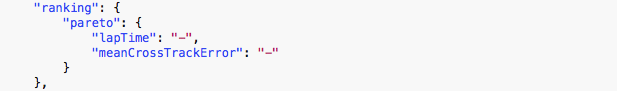
\includegraphics[scale=0.55]{figures/dse/config-ranking}
	\caption{Defining parameters and their preferred directions for ranking.}\label{fig:dse:edit:ranking}
\end{figure}
%
%
%
\subsubsection{Scenario List}\label{sec:dse:edit:scenarios}
Changing a scenario may involve changing one or more different parts of the multi-model and its analysis, such as the specific FMUs used, parameters passed to an FMU, the multi-model the DSE is based upon, along with any data files used by the objective scripts (Section~\ref{sec:dse:edit:objectivesexternal}) to evaluate performance.  This feature is currently under development and so only the objective data file selection is implemented presently. As such, scenarios are simply passed to objectives.

Combining all these sections results in a complete DSE configuration, as shown in Figure~\ref{fig:dse:edit:whole}.
%
%
%
\begin{figure}[ht]
	\centering
	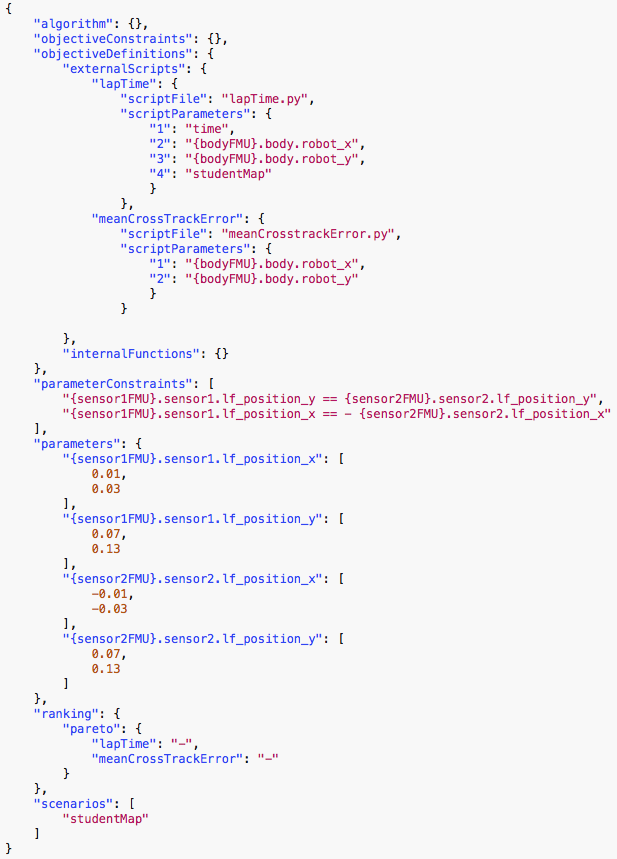
\includegraphics[scale=0.55]{figures/dse/config-whole}
		\caption{A complete DSE configuration for the Line Follower Robot example.}\label{fig:dse:edit:whole}
\end{figure}